
%% $Id$

\documentclass[12pt,a4paper,fleqn]{report}
\usepackage{latexsym,graphicx}
\usepackage{listings}
\usepackage[refpage]{nomencl}
\usepackage{../../iman,../../extra,../../isar,../../proof}
\usepackage{Thy/document/isabelle,Thy/document/isabellesym}
\usepackage{style}
\usepackage{Thy/document/pdfsetup}

\newcommand{\cmd}[1]{\isacommand{#1}}

\newcommand{\isasymINFIX}{\cmd{infix}}
\newcommand{\isasymLOCALE}{\cmd{locale}}
\newcommand{\isasymINCLUDES}{\cmd{includes}}
\newcommand{\isasymDATATYPE}{\cmd{datatype}}
\newcommand{\isasymAXCLASS}{\cmd{axclass}}
\newcommand{\isasymFIXES}{\cmd{fixes}}
\newcommand{\isasymASSUMES}{\cmd{assumes}}
\newcommand{\isasymDEFINES}{\cmd{defines}}
\newcommand{\isasymNOTES}{\cmd{notes}}
\newcommand{\isasymSHOWS}{\cmd{shows}}
\newcommand{\isasymCLASS}{\cmd{class}}
\newcommand{\isasymINSTANCE}{\cmd{instance}}
\newcommand{\isasymLEMMA}{\cmd{lemma}}
\newcommand{\isasymPROOF}{\cmd{proof}}
\newcommand{\isasymQED}{\cmd{qed}}
\newcommand{\isasymFIX}{\cmd{fix}}
\newcommand{\isasymASSUME}{\cmd{assume}}
\newcommand{\isasymSHOW}{\cmd{show}}
\newcommand{\isasymNOTE}{\cmd{note}}
\newcommand{\isasymEXPORTCODE}{\cmd{export\_code}}
\newcommand{\isasymCODEDATATYPE}{\cmd{code\_datatype}}
\newcommand{\isasymCODECONST}{\cmd{code\_const}}
\newcommand{\isasymCODETYPE}{\cmd{code\_type}}
\newcommand{\isasymCODECLASS}{\cmd{code\_class}}
\newcommand{\isasymCODEINSTANCE}{\cmd{code\_instance}}
\newcommand{\isasymCODERESERVED}{\cmd{code\_reserved}}
\newcommand{\isasymCODEMODULENAME}{\cmd{code\_modulename}}
\newcommand{\isasymCODEMODULEPROLOG}{\cmd{code\_moduleprolog}}
\newcommand{\isasymCODEAXIOMS}{\cmd{code\_axioms}}
\newcommand{\isasymCODEABSTYPE}{\cmd{code\_abstype}}
\newcommand{\isasymPRINTCODESETUP}{\cmd{print\_codesetup}}
\newcommand{\isasymPRINTCLASSES}{\cmd{print\_classes}}
\newcommand{\isasymCODETHMS}{\cmd{code\_thms}}
\newcommand{\isasymCODEDEPS}{\cmd{code\_deps}}
\newcommand{\isasymFUN}{\cmd{fun}}
\newcommand{\isasymFUNCTION}{\cmd{function}}
\newcommand{\isasymPRIMREC}{\cmd{primrec}}
\newcommand{\isasymCONSTDEFS}{\cmd{constdefs}}
\newcommand{\isasymRECDEF}{\cmd{recdef}}

\isakeeptag{tt}
\renewcommand{\isatagtt}{\isabellestyle{tt}\isastyle}
\renewcommand{\endisatagtt}{\isabellestyle{it}\isastyle}

\newcommand{\qt}[1]{``#1''}
\newcommand{\qtt}[1]{"{}{#1}"{}}
\newcommand{\qn}[1]{\emph{#1}}
\newcommand{\strong}[1]{{\bfseries #1}}
\newcommand{\fixme}[1][!]{\strong{FIXME: #1}}

\lstset{basicstyle=\scriptsize\ttfamily,keywordstyle=\itshape,commentstyle=\itshape\sffamily,frame=single}
\newcommand{\lstsml}[1]{\lstset{language=ML}\lstinputlisting{#1}}
\newcommand{\lsthaskell}[1]{\lstset{language=Haskell}\lstinputlisting{#1}}

\hyphenation{Isabelle}
\hyphenation{Isar}

\isadroptag{theory}
\title{
\includegraphics[scale=0.5]{isabelle_isar}
  \\[4ex] Code generation from Isabelle/HOL theories}
\author{\emph{Florian Haftmann}}


\begin{document}

\maketitle

\begin{abstract}
  This tutorial gives a motivation-driven introduction
  to a generic code generator framework in Isabelle
  for generating executable code in functional
  programming languages from logical specifications.
\end{abstract}

\thispagestyle{empty}\clearpage

\pagenumbering{roman}
\clearfirst

%
\begin{isabellebody}%
\def\isabellecontext{Codegen}%
%
\isadelimtheory
\isanewline
%
\endisadelimtheory
%
\isatagtheory
%
\endisatagtheory
{\isafoldtheory}%
%
\isadelimtheory
%
\endisadelimtheory
%
\isadelimML
%
\endisadelimML
%
\isatagML
%
\endisatagML
{\isafoldML}%
%
\isadelimML
%
\endisadelimML
%
\isamarkupchapter{Code generation from Isabelle theories%
}
\isamarkuptrue%
%
\isamarkupsection{Introduction%
}
\isamarkuptrue%
%
\isamarkupsubsection{Motivation%
}
\isamarkuptrue%
%
\begin{isamarkuptext}%
Executing formal specifications as programs is a well-established
  topic in the theorem proving community.  With increasing
  application of theorem proving systems in the area of
  software development and verification, its relevance manifests
  for running test cases and rapid prototyping.  In logical
  calculi like constructive type theory,
  a notion of executability is implicit due to the nature
  of the calculus.  In contrast, specifications in Isabelle/HOL
  can be highly non-executable.  In order to bridge
  the gap between logic and executable specifications,
  an explicit non-trivial transformation has to be applied:
  code generation.

  This tutorial introduces a generic code generator for the
  Isabelle system \cite{isa-tutorial}.
  Generic in the sense that the
  \qn{target language} for which code shall ultimately be
  generated is not fixed but may be an arbitrary state-of-the-art
  functional programming language (currently, the implementation
  supports SML \cite{SML}, OCaml \cite{OCaml} and Haskell \cite{haskell-revised-report}).
  We aim to provide a
  versatile environment
  suitable for software development and verification,
  structuring the process
  of code generation into a small set of orthogonal principles
  while achieving a big coverage of application areas
  with maximum flexibility.

  For readers, some familiarity and experience
  with the ingredients
  of the HOL \emph{Main} theory is assumed.%
\end{isamarkuptext}%
\isamarkuptrue%
%
\isamarkupsubsection{Overview%
}
\isamarkuptrue%
%
\begin{isamarkuptext}%
The code generator aims to be usable with no further ado
  in most cases while allowing for detailed customization.
  This manifests in the structure of this tutorial: this introduction
  continues with a short introduction of concepts.  Section
  \secref{sec:basics} explains how to use the framework naively,
  presuming a reasonable default setup.  Then, section
  \secref{sec:advanced} deals with advanced topics,
  introducing further aspects of the code generator framework
  in a motivation-driven manner.  Last, section \secref{sec:ml}
  introduces the framework's internal programming interfaces.

  \begin{warn}
    Ultimately, the code generator which this tutorial deals with
    is supposed to replace the already established code generator
    by Stefan Berghofer \cite{Berghofer-Nipkow:2002}.
    So, for the moment, there are two distinct code generators
    in Isabelle.
    Also note that while the framework itself is largely
    object-logic independent, only HOL provides a reasonable
    framework setup.    
  \end{warn}%
\end{isamarkuptext}%
\isamarkuptrue%
%
\isamarkupsubsection{Code generation process%
}
\isamarkuptrue%
%
\begin{isamarkuptext}%
\begin{figure}[h]
  \centering
  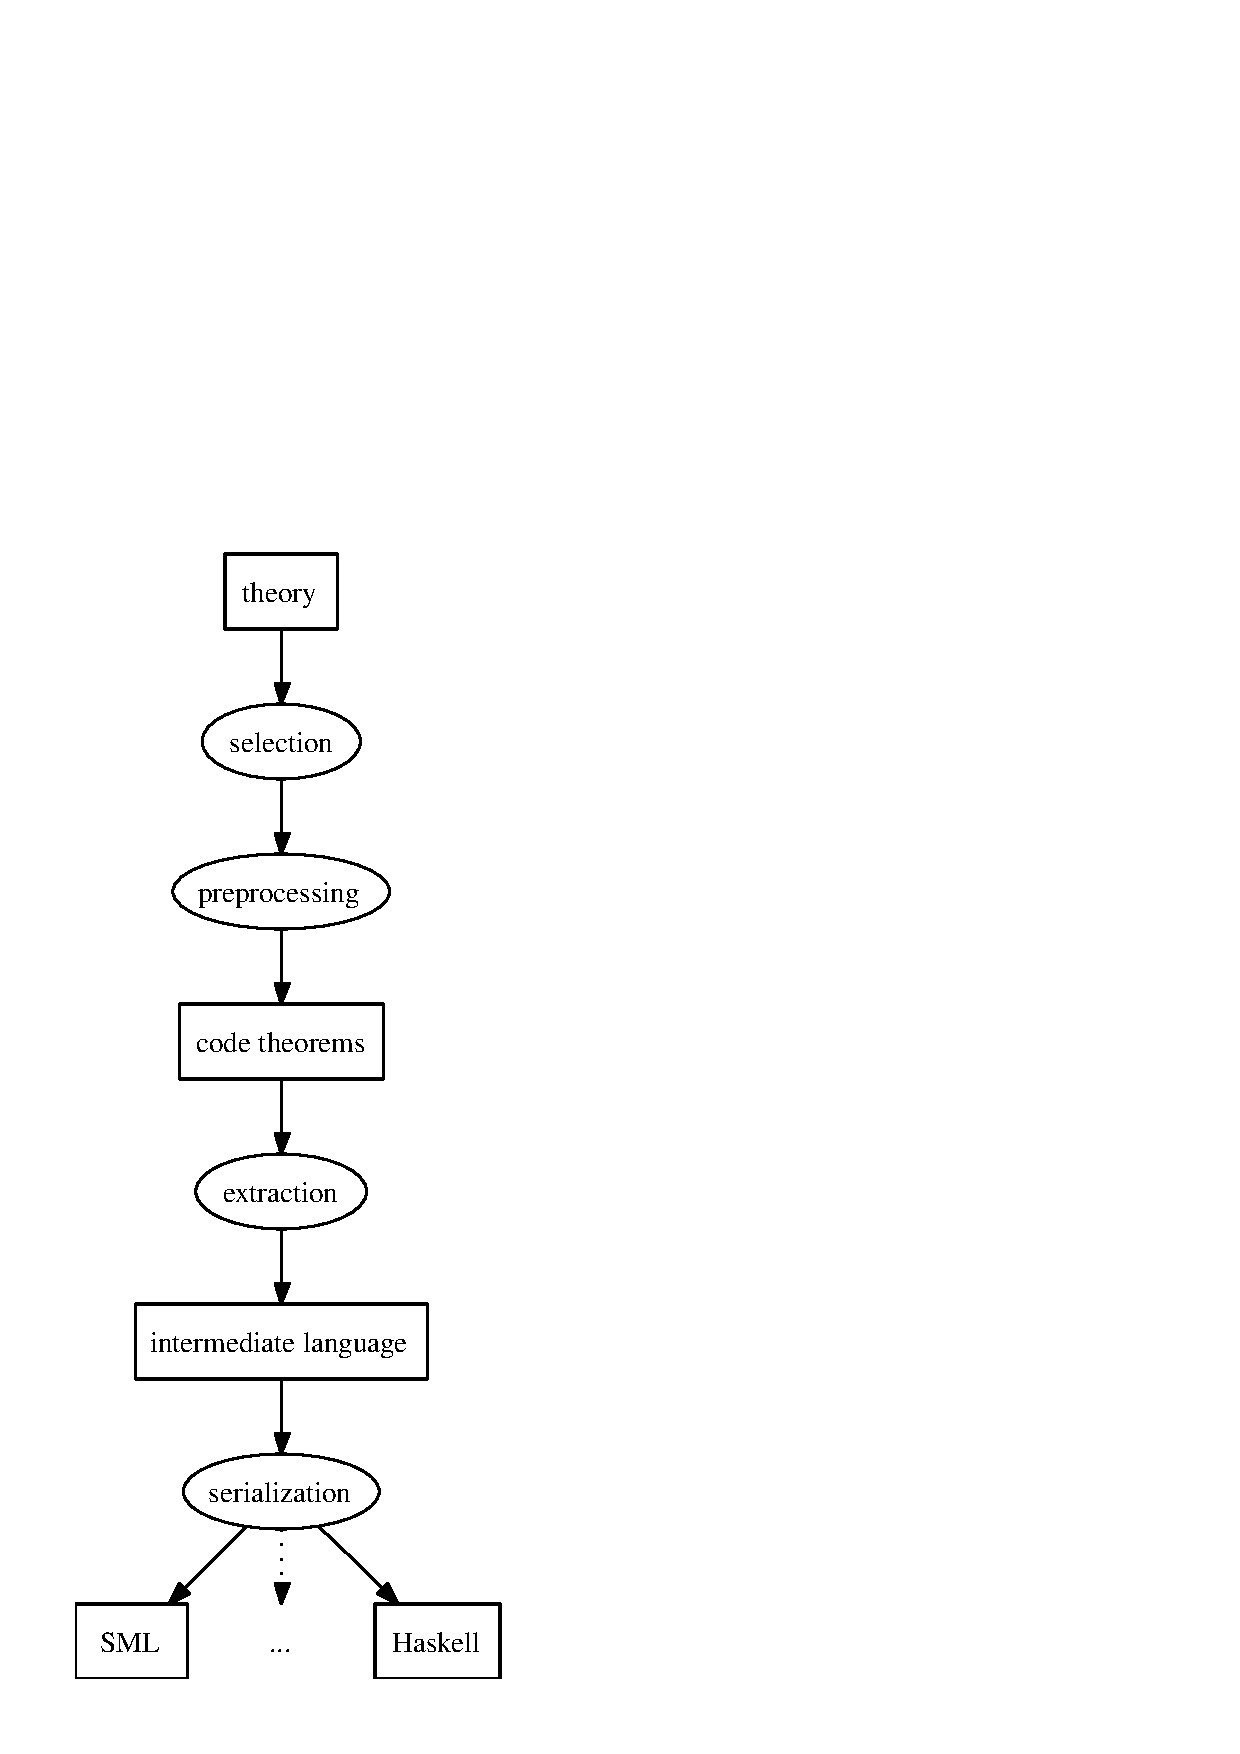
\includegraphics[width=0.7\textwidth]{codegen_process}
  \caption{code generator -- processing overview}
  \label{fig:process}
  \end{figure}

  The code generator employs a notion of executability
  for three foundational executable ingredients known
  from functional programming:
  \emph{defining equations}, \emph{datatypes}, and
  \emph{type classes}. A defining equation as a first approximation
  is a theorem of the form \isa{f\ t\isactrlisub {\isadigit{1}}\ t\isactrlisub {\isadigit{2}}\ {\isasymdots}\ t\isactrlisub n\ {\isasymequiv}\ t}
  (an equation headed by a constant \isa{f} with arguments
  \isa{t\isactrlisub {\isadigit{1}}\ t\isactrlisub {\isadigit{2}}\ {\isasymdots}\ t\isactrlisub n} and right hand side \isa{t}.
  Code generation aims to turn defining equations
  into a functional program by running through
  a process (see figure \ref{fig:process}):

  \begin{itemize}

    \item Out of the vast collection of theorems proven in a
      \qn{theory}, a reasonable subset modeling
      defining equations is \qn{selected}.

    \item On those selected theorems, certain
      transformations are carried out
      (\qn{preprocessing}).  Their purpose is to turn theorems
      representing non- or badly executable
      specifications into equivalent but executable counterparts.
      The result is a structured collection of \qn{code theorems}.

    \item These \qn{code theorems} then are extracted
      into an Haskell-like intermediate
      language.

    \item Finally, out of the intermediate language the final
      code in the desired \qn{target language} is \qn{serialized}.

  \end{itemize}

  From these steps, only the two last are carried out
  outside the logic; by keeping this layer as
  thin as possible, the amount of code to trust is
  kept to a minimum.%
\end{isamarkuptext}%
\isamarkuptrue%
%
\isamarkupsection{Basics \label{sec:basics}%
}
\isamarkuptrue%
%
\isamarkupsubsection{Invoking the code generator%
}
\isamarkuptrue%
%
\begin{isamarkuptext}%
Thanks to a reasonable setup of the HOL theories, in
  most cases code generation proceeds without further ado:%
\end{isamarkuptext}%
\isamarkuptrue%
\isacommand{consts}\isamarkupfalse%
\isanewline
\ \ fac\ {\isacharcolon}{\isacharcolon}\ {\isachardoublequoteopen}nat\ {\isasymRightarrow}\ nat{\isachardoublequoteclose}\isanewline
\isanewline
\isacommand{primrec}\isamarkupfalse%
\isanewline
\ \ {\isachardoublequoteopen}fac\ {\isadigit{0}}\ {\isacharequal}\ {\isadigit{1}}{\isachardoublequoteclose}\isanewline
\ \ {\isachardoublequoteopen}fac\ {\isacharparenleft}Suc\ n{\isacharparenright}\ {\isacharequal}\ Suc\ n\ {\isacharasterisk}\ fac\ n{\isachardoublequoteclose}%
\begin{isamarkuptext}%
This executable specification is now turned to SML code:%
\end{isamarkuptext}%
\isamarkuptrue%
\isacommand{code{\isacharunderscore}gen}\isamarkupfalse%
\ fac\ {\isacharparenleft}SML\ {\isachardoublequoteopen}examples{\isacharslash}fac{\isachardot}ML{\isachardoublequoteclose}{\isacharparenright}%
\begin{isamarkuptext}%
The \isa{{\isasymCODEGEN}} command takes a space-separated list of
  constants together with \qn{serialization directives}
  in parentheses. These start with a \qn{target language}
  identifier, followed by arguments, their semantics
  depending on the target. In the SML case, a filename
  is given where to write the generated code to.

  Internally, the defining equations for all selected
  constants are taken, including any transitively required
  constants, datatypes and classes, resulting in the following
  code:

  \lstsml{Thy/examples/fac.ML}

  The code generator will complain when a required
  ingredient does not provide a executable counterpart.
  This is the case if an involved type is not a datatype:%
\end{isamarkuptext}%
\isamarkuptrue%
%
\isadelimML
%
\endisadelimML
%
\isatagML
%
\endisatagML
{\isafoldML}%
%
\isadelimML
\isanewline
%
\endisadelimML
\isacommand{typedecl}\isamarkupfalse%
\ {\isacharprime}a\ foo\isanewline
\isanewline
\isacommand{definition}\isamarkupfalse%
\isanewline
\ \ bar\ {\isacharcolon}{\isacharcolon}\ {\isachardoublequoteopen}{\isacharprime}a\ foo\ {\isasymRightarrow}\ {\isacharprime}a\ {\isasymRightarrow}\ {\isacharprime}a{\isachardoublequoteclose}\ \isakeyword{where}\isanewline
\ \ {\isachardoublequoteopen}bar\ x\ y\ {\isacharequal}\ y{\isachardoublequoteclose}\isanewline
%
\isadelimML
%
\endisadelimML
%
\isatagML
%
\endisatagML
{\isafoldML}%
%
\isadelimML
%
\endisadelimML
\isanewline
\isacommand{code{\isacharunderscore}gen}\isamarkupfalse%
\ bar\ {\isacharparenleft}SML\ {\isachardoublequoteopen}examples{\isacharslash}fail{\isacharunderscore}type{\isachardot}ML{\isachardoublequoteclose}{\isacharparenright}%
\begin{isamarkuptext}%
\noindent will result in an error. Likewise, generating code
  for constants not yielding
  a defining equation will fail, e.g.~the Hilbert choice
  operation \isa{SOME}:%
\end{isamarkuptext}%
\isamarkuptrue%
%
\isadelimML
%
\endisadelimML
%
\isatagML
%
\endisatagML
{\isafoldML}%
%
\isadelimML
\isanewline
%
\endisadelimML
\isacommand{definition}\isamarkupfalse%
\isanewline
\ \ pick{\isacharunderscore}some\ {\isacharcolon}{\isacharcolon}\ {\isachardoublequoteopen}{\isacharprime}a\ list\ {\isasymRightarrow}\ {\isacharprime}a{\isachardoublequoteclose}\ \isakeyword{where}\isanewline
\ \ {\isachardoublequoteopen}pick{\isacharunderscore}some\ xs\ {\isacharequal}\ {\isacharparenleft}SOME\ x{\isachardot}\ x\ {\isasymin}\ set\ xs{\isacharparenright}{\isachardoublequoteclose}\isanewline
%
\isadelimML
%
\endisadelimML
%
\isatagML
%
\endisatagML
{\isafoldML}%
%
\isadelimML
%
\endisadelimML
\isanewline
\isacommand{code{\isacharunderscore}gen}\isamarkupfalse%
\ pick{\isacharunderscore}some\ {\isacharparenleft}SML\ {\isachardoublequoteopen}examples{\isacharslash}fail{\isacharunderscore}const{\isachardot}ML{\isachardoublequoteclose}{\isacharparenright}%
\isamarkupsubsection{Theorem selection%
}
\isamarkuptrue%
%
\begin{isamarkuptext}%
The list of all defining equations in a theory may be inspected
  using the \isa{{\isasymPRINTCODESETUP}} command:%
\end{isamarkuptext}%
\isamarkuptrue%
\isacommand{print{\isacharunderscore}codesetup}\isamarkupfalse%
%
\begin{isamarkuptext}%
\noindent which displays a table of constant with corresponding
  defining equations (the additional stuff displayed
  shall not bother us for the moment). If this table does
  not provide at least one function
  equation, the table of primitive definitions is searched
  whether it provides one.

  The typical HOL tools are already set up in a way that
  function definitions introduced by \isa{{\isasymFUN}},
  \isa{{\isasymFUNCTION}}, \isa{{\isasymPRIMREC}}
  \isa{{\isasymRECDEF}} are implicitly propagated
  to this defining equation table. Specific theorems may be
  selected using an attribute: \emph{code func}. As example,
  a weight selector function:%
\end{isamarkuptext}%
\isamarkuptrue%
\isacommand{consts}\isamarkupfalse%
\isanewline
\ \ pick\ {\isacharcolon}{\isacharcolon}\ {\isachardoublequoteopen}{\isacharparenleft}nat\ {\isasymtimes}\ {\isacharprime}a{\isacharparenright}\ list\ {\isasymRightarrow}\ nat\ {\isasymRightarrow}\ {\isacharprime}a{\isachardoublequoteclose}\isanewline
\isanewline
\isacommand{primrec}\isamarkupfalse%
\isanewline
\ \ {\isachardoublequoteopen}pick\ {\isacharparenleft}x{\isacharhash}xs{\isacharparenright}\ n\ {\isacharequal}\ {\isacharparenleft}let\ {\isacharparenleft}k{\isacharcomma}\ v{\isacharparenright}\ {\isacharequal}\ x\ in\isanewline
\ \ \ \ if\ n\ {\isacharless}\ k\ then\ v\ else\ pick\ xs\ {\isacharparenleft}n\ {\isacharminus}\ k{\isacharparenright}{\isacharparenright}{\isachardoublequoteclose}%
\begin{isamarkuptext}%
We want to eliminate the explicit destruction
  of \isa{x} to \isa{{\isacharparenleft}k{\isacharcomma}\ v{\isacharparenright}}:%
\end{isamarkuptext}%
\isamarkuptrue%
\isacommand{lemma}\isamarkupfalse%
\ {\isacharbrackleft}code\ func{\isacharbrackright}{\isacharcolon}\isanewline
\ \ {\isachardoublequoteopen}pick\ {\isacharparenleft}{\isacharparenleft}k{\isacharcomma}\ v{\isacharparenright}{\isacharhash}xs{\isacharparenright}\ n\ {\isacharequal}\ {\isacharparenleft}if\ n\ {\isacharless}\ k\ then\ v\ else\ pick\ xs\ {\isacharparenleft}n\ {\isacharminus}\ k{\isacharparenright}{\isacharparenright}{\isachardoublequoteclose}\isanewline
%
\isadelimproof
\ \ %
\endisadelimproof
%
\isatagproof
\isacommand{by}\isamarkupfalse%
\ simp%
\endisatagproof
{\isafoldproof}%
%
\isadelimproof
\isanewline
%
\endisadelimproof
\isanewline
\isacommand{code{\isacharunderscore}gen}\isamarkupfalse%
\ pick\ {\isacharparenleft}SML\ {\isachardoublequoteopen}examples{\isacharslash}pick{\isadigit{1}}{\isachardot}ML{\isachardoublequoteclose}{\isacharparenright}%
\begin{isamarkuptext}%
This theorem is now added to the defining equation table:

  \lstsml{Thy/examples/pick1.ML}

  It might be convenient to remove the pointless original
  equation, using the \emph{nofunc} attribute:%
\end{isamarkuptext}%
\isamarkuptrue%
\isacommand{lemmas}\isamarkupfalse%
\ {\isacharbrackleft}code\ nofunc{\isacharbrackright}\ {\isacharequal}\ pick{\isachardot}simps\ \isanewline
\isanewline
\isacommand{code{\isacharunderscore}gen}\isamarkupfalse%
\ pick\ {\isacharparenleft}SML\ {\isachardoublequoteopen}examples{\isacharslash}pick{\isadigit{2}}{\isachardot}ML{\isachardoublequoteclose}{\isacharparenright}%
\begin{isamarkuptext}%
\lstsml{Thy/examples/pick2.ML}

  Syntactic redundancies are implicitly dropped. For example,
  using a modified version of the \isa{fac} function
  as defining equation, the then redundant (since
  syntactically subsumed) original defining equations
  are dropped, resulting in a warning:%
\end{isamarkuptext}%
\isamarkuptrue%
\isacommand{lemma}\isamarkupfalse%
\ {\isacharbrackleft}code\ func{\isacharbrackright}{\isacharcolon}\isanewline
\ \ {\isachardoublequoteopen}fac\ n\ {\isacharequal}\ {\isacharparenleft}case\ n\ of\ {\isadigit{0}}\ {\isasymRightarrow}\ {\isadigit{1}}\ {\isacharbar}\ Suc\ m\ {\isasymRightarrow}\ n\ {\isacharasterisk}\ fac\ m{\isacharparenright}{\isachardoublequoteclose}\isanewline
%
\isadelimproof
\ \ %
\endisadelimproof
%
\isatagproof
\isacommand{by}\isamarkupfalse%
\ {\isacharparenleft}cases\ n{\isacharparenright}\ simp{\isacharunderscore}all%
\endisatagproof
{\isafoldproof}%
%
\isadelimproof
\isanewline
%
\endisadelimproof
\isanewline
\isacommand{code{\isacharunderscore}gen}\isamarkupfalse%
\ fac\ {\isacharparenleft}SML\ {\isachardoublequoteopen}examples{\isacharslash}fac{\isacharunderscore}case{\isachardot}ML{\isachardoublequoteclose}{\isacharparenright}%
\begin{isamarkuptext}%
\lstsml{Thy/examples/fac_case.ML}

  \begin{warn}
    The attributes \emph{code} and \emph{code del}
    associated with the existing code generator also apply to
    the new one: \emph{code} implies \emph{code func},
    and \emph{code del} implies \emph{code nofunc}.
  \end{warn}%
\end{isamarkuptext}%
\isamarkuptrue%
%
\isamarkupsubsection{Type classes%
}
\isamarkuptrue%
%
\begin{isamarkuptext}%
Type classes enter the game via the Isar class package.
  For a short introduction how to use it, see \cite{isabelle-classes};
  here we just illustrate its impact on code generation.

  In a target language, type classes may be represented
  natively (as in the case of Haskell). For languages
  like SML, they are implemented using \emph{dictionaries}.
  Our following example specifies a class \qt{null},
  assigning to each of its inhabitants a \qt{null} value:%
\end{isamarkuptext}%
\isamarkuptrue%
\isacommand{class}\isamarkupfalse%
\ null\ {\isacharequal}\isanewline
\ \ \isakeyword{fixes}\ null\ {\isacharcolon}{\isacharcolon}\ {\isacharprime}a\isanewline
\isanewline
\isacommand{consts}\isamarkupfalse%
\isanewline
\ \ head\ {\isacharcolon}{\isacharcolon}\ {\isachardoublequoteopen}{\isacharprime}a{\isasymColon}null\ list\ {\isasymRightarrow}\ {\isacharprime}a{\isachardoublequoteclose}\isanewline
\isanewline
\isacommand{primrec}\isamarkupfalse%
\isanewline
\ \ {\isachardoublequoteopen}head\ {\isacharbrackleft}{\isacharbrackright}\ {\isacharequal}\ null{\isachardoublequoteclose}\isanewline
\ \ {\isachardoublequoteopen}head\ {\isacharparenleft}x{\isacharhash}xs{\isacharparenright}\ {\isacharequal}\ x{\isachardoublequoteclose}%
\begin{isamarkuptext}%
We provide some instances for our \isa{null}:%
\end{isamarkuptext}%
\isamarkuptrue%
\isacommand{instance}\isamarkupfalse%
\ option\ {\isacharcolon}{\isacharcolon}\ {\isacharparenleft}type{\isacharparenright}\ null\isanewline
\ \ {\isachardoublequoteopen}null\ {\isasymequiv}\ None{\isachardoublequoteclose}%
\isadelimproof
\ %
\endisadelimproof
%
\isatagproof
\isacommand{{\isachardot}{\isachardot}}\isamarkupfalse%
%
\endisatagproof
{\isafoldproof}%
%
\isadelimproof
%
\endisadelimproof
\isanewline
\isanewline
\isacommand{instance}\isamarkupfalse%
\ list\ {\isacharcolon}{\isacharcolon}\ {\isacharparenleft}type{\isacharparenright}\ null\isanewline
\ \ {\isachardoublequoteopen}null\ {\isasymequiv}\ {\isacharbrackleft}{\isacharbrackright}{\isachardoublequoteclose}%
\isadelimproof
\ %
\endisadelimproof
%
\isatagproof
\isacommand{{\isachardot}{\isachardot}}\isamarkupfalse%
%
\endisatagproof
{\isafoldproof}%
%
\isadelimproof
%
\endisadelimproof
%
\begin{isamarkuptext}%
Constructing a dummy example:%
\end{isamarkuptext}%
\isamarkuptrue%
\isacommand{definition}\isamarkupfalse%
\isanewline
\ \ {\isachardoublequoteopen}dummy\ {\isacharequal}\ head\ {\isacharbrackleft}Some\ {\isacharparenleft}Suc\ {\isadigit{0}}{\isacharparenright}{\isacharcomma}\ None{\isacharbrackright}{\isachardoublequoteclose}%
\begin{isamarkuptext}%
Type classes offer a suitable occasion to introduce
  the Haskell serializer.  Its usage is almost the same
  as SML, but, in accordance with conventions
  some Haskell systems enforce, each module ends
  up in a single file. The module hierarchy is reflected in
  the file system, with root given by the user.%
\end{isamarkuptext}%
\isamarkuptrue%
\isacommand{code{\isacharunderscore}gen}\isamarkupfalse%
\ dummy\ {\isacharparenleft}Haskell\ {\isachardoublequoteopen}examples{\isacharslash}{\isachardoublequoteclose}{\isacharparenright}%
\begin{isamarkuptext}%
\lsthaskell{Thy/examples/Codegen.hs}

  (we have left out all other modules).

  The whole code in SML with explicit dictionary passing:%
\end{isamarkuptext}%
\isamarkuptrue%
\isacommand{code{\isacharunderscore}gen}\isamarkupfalse%
\ dummy\ {\isacharparenleft}SML\ {\isachardoublequoteopen}examples{\isacharslash}class{\isachardot}ML{\isachardoublequoteclose}{\isacharparenright}%
\begin{isamarkuptext}%
\lstsml{Thy/examples/class.ML}%
\end{isamarkuptext}%
\isamarkuptrue%
%
\begin{isamarkuptext}%
or in OCaml:%
\end{isamarkuptext}%
\isamarkuptrue%
\isacommand{code{\isacharunderscore}gen}\isamarkupfalse%
\ dummy\ {\isacharparenleft}OCaml\ {\isachardoublequoteopen}examples{\isacharslash}class{\isachardot}ocaml{\isachardoublequoteclose}{\isacharparenright}%
\begin{isamarkuptext}%
\lstsml{Thy/examples/class.ocaml}%
\end{isamarkuptext}%
\isamarkuptrue%
%
\isamarkupsubsection{Incremental code generation%
}
\isamarkuptrue%
%
\begin{isamarkuptext}%
Code generation is \emph{incremental}: theorems
  and abstract intermediate code are cached and extended on demand.
  The cache may be partially or fully dropped if the underlying
  executable content of the theory changes.
  Implementation of caching is supposed to transparently
  hid away the details from the user.  Anyway, caching
  reaches the surface by using a slightly more general form
  of the \isa{{\isasymCODEGEN}}: either the list of constants or the
  list of serialization expressions may be dropped.  If no
  serialization expressions are given, only abstract code
  is generated and cached; if no constants are given, the
  current cache is serialized.

  For explorative purpose, the
  \isa{{\isasymCODETHMS}} command may prove useful:%
\end{isamarkuptext}%
\isamarkuptrue%
\isacommand{code{\isacharunderscore}thms}\isamarkupfalse%
%
\begin{isamarkuptext}%
\noindent print all cached defining equations (i.e.~\emph{after}
  any applied transformation).  A
  list of constants may be given; their function
  equations are added to the cache if not already present.%
\end{isamarkuptext}%
\isamarkuptrue%
%
\isamarkupsection{Recipes and advanced topics \label{sec:advanced}%
}
\isamarkuptrue%
%
\begin{isamarkuptext}%
In this tutorial, we do not attempt to give an exhaustive
  description of the code generator framework; instead,
  we cast a light on advanced topics by introducing
  them together with practically motivated examples.  Concerning
  further reading, see

  \begin{itemize}

  \item the Isabelle/Isar Reference Manual \cite{isabelle-isar-ref}
    for exhaustive syntax diagrams.
  \item or \fixme[ref] which deals with foundational issues
    of the code generator framework.

  \end{itemize}%
\end{isamarkuptext}%
\isamarkuptrue%
%
\isamarkupsubsection{Library theories%
}
\isamarkuptrue%
%
\begin{isamarkuptext}%
The HOL \emph{Main} theory already provides a code generator setup
  which should be suitable for most applications. Common extensions
  and modifications are available by certain theories of the HOL
  library; beside being useful in applications, they may serve
  as a tutorial for customizing the code generator setup.

  \begin{description}

    \item[\isa{ExecutableSet}] allows to generate code
       for finite sets using lists.
    \item[\isa{ExecutableRat}] \label{exec_rat} implements rational
       numbers as triples \isa{{\isacharparenleft}sign{\isacharcomma}\ enumerator{\isacharcomma}\ denominator{\isacharparenright}}.
    \item[\isa{EfficientNat}] \label{eff_nat} implements natural numbers by integers,
       which in general will result in higher efficency; pattern
       matching with \isa{{\isadigit{0}}} / \isa{Suc}
       is eliminated.
    \item[\isa{MLString}] provides an additional datatype \isa{mlstring};
       in the HOL default setup, strings in HOL are mapped to list
       of chars in SML; values of type \isa{mlstring} are
       mapped to strings in SML.

  \end{description}%
\end{isamarkuptext}%
\isamarkuptrue%
%
\isamarkupsubsection{Preprocessing%
}
\isamarkuptrue%
%
\begin{isamarkuptext}%
Before selected function theorems are turned into abstract
  code, a chain of definitional transformation steps is carried
  out: \emph{preprocessing}. There are three possibilities
  to customize preprocessing: \emph{inline theorems},
  \emph{inline procedures} and \emph{generic preprocessors}.

  \emph{Inline theorems} are rewriting rules applied to each
  defining equation.  Due to the interpretation of theorems
  of defining equations, rewrites are applied to the right
  hand side and the arguments of the left hand side of an
  equation, but never to the constant heading the left hand side.
  Inline theorems may be declared an undeclared using the
  \emph{code inline} or \emph{code noinline} attribute respectively.

  Some common applications:%
\end{isamarkuptext}%
\isamarkuptrue%
%
\begin{itemize}
     \item replacing non-executable constructs by executable ones: \\
\isacommand{lemma}\isamarkupfalse%
\ {\isacharbrackleft}code\ inline{\isacharbrackright}{\isacharcolon}\isanewline
\ \ {\isachardoublequoteopen}x\ {\isasymin}\ set\ xs\ {\isasymlongleftrightarrow}\ x\ mem\ xs{\isachardoublequoteclose}%
\isadelimproof
\ %
\endisadelimproof
%
\isatagproof
\isacommand{by}\isamarkupfalse%
\ {\isacharparenleft}induct\ xs{\isacharparenright}\ simp{\isacharunderscore}all%
\endisatagproof
{\isafoldproof}%
%
\isadelimproof
%
\endisadelimproof
%
\item eliminating superfluous constants: \\
\isacommand{lemma}\isamarkupfalse%
\ {\isacharbrackleft}code\ inline{\isacharbrackright}{\isacharcolon}\isanewline
\ \ {\isachardoublequoteopen}{\isadigit{1}}\ {\isacharequal}\ Suc\ {\isadigit{0}}{\isachardoublequoteclose}%
\isadelimproof
\ %
\endisadelimproof
%
\isatagproof
\isacommand{by}\isamarkupfalse%
\ simp%
\endisatagproof
{\isafoldproof}%
%
\isadelimproof
%
\endisadelimproof
%
\item replacing executable but inconvenient constructs: \\
\isacommand{lemma}\isamarkupfalse%
\ {\isacharbrackleft}code\ inline{\isacharbrackright}{\isacharcolon}\isanewline
\ \ {\isachardoublequoteopen}xs\ {\isacharequal}\ {\isacharbrackleft}{\isacharbrackright}\ {\isasymlongleftrightarrow}\ List{\isachardot}null\ xs{\isachardoublequoteclose}%
\isadelimproof
\ %
\endisadelimproof
%
\isatagproof
\isacommand{by}\isamarkupfalse%
\ {\isacharparenleft}induct\ xs{\isacharparenright}\ simp{\isacharunderscore}all%
\endisatagproof
{\isafoldproof}%
%
\isadelimproof
%
\endisadelimproof
%
\end{itemize}
%
\begin{isamarkuptext}%
The current set of inline theorems may be inspected using
  the \isa{{\isasymPRINTCODESETUP}} command.

  \emph{Inline procedures} are a generalized version of inline
  theorems written in ML -- rewrite rules are generated dependent
  on the function theorems for a certain function.  One
  application is the implicit expanding of \isa{nat} numerals
  to \isa{{\isadigit{0}}} / \isa{Suc} representation.  See further
  \secref{sec:ml}

  \emph{Generic preprocessors} provide a most general interface,
  transforming a list of function theorems to another
  list of function theorems, provided that neither the heading
  constant nor its type change.  The \isa{{\isadigit{0}}} / \isa{Suc}
  pattern elimination implemented in
  theory \isa{EfficientNat} (\secref{eff_nat}) uses this
  interface.

  \begin{warn}
    The order in which single preprocessing steps are carried
    out currently is not specified; in particular, preprocessing
    is \emph{no} fix point process.  Keep this in mind when
    setting up the preprocessor.

    Further, the attribute \emph{code unfold}
    associated with the existing code generator also applies to
    the new one: \emph{code unfold} implies \emph{code inline}.
  \end{warn}%
\end{isamarkuptext}%
\isamarkuptrue%
%
\isamarkupsubsection{Customizing serialization%
}
\isamarkuptrue%
%
\begin{isamarkuptext}%
Consider the following function and its corresponding
  SML code:%
\end{isamarkuptext}%
\isamarkuptrue%
\isacommand{fun}\isamarkupfalse%
\isanewline
\ \ in{\isacharunderscore}interval\ {\isacharcolon}{\isacharcolon}\ {\isachardoublequoteopen}nat\ {\isasymtimes}\ nat\ {\isasymRightarrow}\ nat\ {\isasymRightarrow}\ bool{\isachardoublequoteclose}\ \isakeyword{where}\isanewline
\ \ {\isachardoublequoteopen}in{\isacharunderscore}interval\ {\isacharparenleft}k{\isacharcomma}\ l{\isacharparenright}\ n\ {\isasymlongleftrightarrow}\ k\ {\isasymle}\ n\ {\isasymand}\ n\ {\isasymle}\ l{\isachardoublequoteclose}%
\isadelimtt
%
\endisadelimtt
%
\isatagtt
%
\endisatagtt
{\isafoldtt}%
%
\isadelimtt
\isanewline
%
\endisadelimtt
\isacommand{code{\isacharunderscore}gen}\isamarkupfalse%
\ in{\isacharunderscore}interval\ {\isacharparenleft}SML\ {\isachardoublequoteopen}examples{\isacharslash}bool{\isacharunderscore}literal{\isachardot}ML{\isachardoublequoteclose}{\isacharparenright}%
\begin{isamarkuptext}%
\lstsml{Thy/examples/bool_literal.ML}

  Though this is correct code, it is a little bit unsatisfactory:
  boolean values and operators are materialized as distinguished
  entities with have nothing to do with the SML-builtin notion
  of \qt{bool}.  This results in less readable code;
  additionally, eager evaluation may cause programs to
  loop or break which would perfectly terminate when
  the existing SML \qt{bool} would be used.  To map
  the HOL \qt{bool} on SML \qt{bool}, we may use
  \qn{custom serializations}:%
\end{isamarkuptext}%
\isamarkuptrue%
%
\isadelimtt
%
\endisadelimtt
%
\isatagtt
\isacommand{code{\isacharunderscore}type}\isamarkupfalse%
\ bool\isanewline
\ \ {\isacharparenleft}SML\ {\isachardoublequoteopen}bool{\isachardoublequoteclose}{\isacharparenright}\isanewline
\isacommand{code{\isacharunderscore}const}\isamarkupfalse%
\ True\ \isakeyword{and}\ False\ \isakeyword{and}\ {\isachardoublequoteopen}op\ {\isasymand}{\isachardoublequoteclose}\isanewline
\ \ {\isacharparenleft}SML\ {\isachardoublequoteopen}true{\isachardoublequoteclose}\ \isakeyword{and}\ {\isachardoublequoteopen}false{\isachardoublequoteclose}\ \isakeyword{and}\ {\isachardoublequoteopen}{\isacharunderscore}\ andalso\ {\isacharunderscore}{\isachardoublequoteclose}{\isacharparenright}%
\endisatagtt
{\isafoldtt}%
%
\isadelimtt
%
\endisadelimtt
%
\begin{isamarkuptext}%
The \isa{{\isasymCODETYPE}} commad takes a type constructor
  as arguments together with a list of custom serializations.
  Each custom serialization starts with a target language
  identifier followed by an expression, which during
  code serialization is inserted whenever the type constructor
  would occur.  For constants, \isa{{\isasymCODECONST}} implements
  the corresponding mechanism.  Each ``\verb|_|'' in
  a serialization expression is treated as a placeholder
  for the type constructor's (the constant's) arguments.%
\end{isamarkuptext}%
\isamarkuptrue%
\isacommand{code{\isacharunderscore}reserved}\isamarkupfalse%
\ SML\isanewline
\ \ bool\ true\ false%
\begin{isamarkuptext}%
To assert that the existing \qt{bool}, \qt{true} and \qt{false}
  is not used for generated code, we use \isa{{\isasymCODERESERVED}}.

  After this setup, code looks quite more readable:%
\end{isamarkuptext}%
\isamarkuptrue%
\isacommand{code{\isacharunderscore}gen}\isamarkupfalse%
\ in{\isacharunderscore}interval\ {\isacharparenleft}SML\ {\isachardoublequoteopen}examples{\isacharslash}bool{\isacharunderscore}mlbool{\isachardot}ML{\isachardoublequoteclose}{\isacharparenright}%
\begin{isamarkuptext}%
\lstsml{Thy/examples/bool_mlbool.ML}

  This still is not perfect: the parentheses
  around the \qt{andalso} expression are superfluous.
  Though the serializer
  by no means attempts to imitate the rich Isabelle syntax
  framework, it provides some common idioms, notably
  associative infixes with precedences which may be used here:%
\end{isamarkuptext}%
\isamarkuptrue%
%
\isadelimtt
%
\endisadelimtt
%
\isatagtt
\isacommand{code{\isacharunderscore}const}\isamarkupfalse%
\ {\isachardoublequoteopen}op\ {\isasymand}{\isachardoublequoteclose}\isanewline
\ \ {\isacharparenleft}SML\ \isakeyword{infixl}\ {\isadigit{1}}\ {\isachardoublequoteopen}andalso{\isachardoublequoteclose}{\isacharparenright}%
\endisatagtt
{\isafoldtt}%
%
\isadelimtt
%
\endisadelimtt
\isanewline
\isanewline
\isacommand{code{\isacharunderscore}gen}\isamarkupfalse%
\ in{\isacharunderscore}interval\ {\isacharparenleft}SML\ {\isachardoublequoteopen}examples{\isacharslash}bool{\isacharunderscore}infix{\isachardot}ML{\isachardoublequoteclose}{\isacharparenright}%
\begin{isamarkuptext}%
\lstsml{Thy/examples/bool_infix.ML}

  Next, we try to map HOL pairs to SML pairs, using the
  infix ``\verb|*|'' type constructor and parentheses:%
\end{isamarkuptext}%
\isamarkuptrue%
\isanewline
%
\isadelimtt
%
\endisadelimtt
%
\isatagtt
\isacommand{code{\isacharunderscore}type}\isamarkupfalse%
\ {\isacharasterisk}\isanewline
\ \ {\isacharparenleft}SML\ \isakeyword{infix}\ {\isadigit{2}}\ {\isachardoublequoteopen}{\isacharasterisk}{\isachardoublequoteclose}{\isacharparenright}\isanewline
\isanewline
\isacommand{code{\isacharunderscore}const}\isamarkupfalse%
\ Pair\isanewline
\ \ {\isacharparenleft}SML\ {\isachardoublequoteopen}{\isacharbang}{\isacharparenleft}{\isacharparenleft}{\isacharunderscore}{\isacharparenright}{\isacharcomma}{\isacharslash}\ {\isacharparenleft}{\isacharunderscore}{\isacharparenright}{\isacharparenright}{\isachardoublequoteclose}{\isacharparenright}%
\endisatagtt
{\isafoldtt}%
%
\isadelimtt
%
\endisadelimtt
%
\begin{isamarkuptext}%
The initial bang ``\verb|!|'' tells the serializer to never put
  parentheses around the whole expression (they are already present),
  while the parentheses around argument place holders
  tell not to put parentheses around the arguments.
  The slash ``\verb|/|'' (followed by arbitrary white space)
  inserts a space which may be used as a break if necessary
  during pretty printing.

  So far, we did only provide more idiomatic serializations for
  constructs which would be executable on their own.  Target-specific
  serializations may also be used to \emph{implement} constructs
  which have no explicit notion of executability.  For example,
  take the HOL integers:%
\end{isamarkuptext}%
\isamarkuptrue%
\isacommand{definition}\isamarkupfalse%
\isanewline
\ \ double{\isacharunderscore}inc\ {\isacharcolon}{\isacharcolon}\ {\isachardoublequoteopen}int\ {\isasymRightarrow}\ int{\isachardoublequoteclose}\ \isakeyword{where}\isanewline
\ \ {\isachardoublequoteopen}double{\isacharunderscore}inc\ k\ {\isacharequal}\ {\isadigit{2}}\ {\isacharasterisk}\ k\ {\isacharplus}\ {\isadigit{1}}{\isachardoublequoteclose}\isanewline
\isanewline
\isacommand{code{\isacharunderscore}gen}\isamarkupfalse%
\ double{\isacharunderscore}inc\ {\isacharparenleft}SML\ {\isachardoublequoteopen}examples{\isacharslash}integers{\isachardot}ML{\isachardoublequoteclose}{\isacharparenright}%
\begin{isamarkuptext}%
will fail: \isa{int} in HOL is implemented using a quotient
  type, which does not provide any notion of executability.
  \footnote{Eventually, we also want to provide executability
  for quotients.}.  However, we could use the SML builtin
  integers:%
\end{isamarkuptext}%
\isamarkuptrue%
%
\isadelimtt
%
\endisadelimtt
%
\isatagtt
\isacommand{code{\isacharunderscore}type}\isamarkupfalse%
\ int\isanewline
\ \ {\isacharparenleft}SML\ {\isachardoublequoteopen}IntInf{\isachardot}int{\isachardoublequoteclose}{\isacharparenright}\isanewline
\isanewline
\isacommand{code{\isacharunderscore}const}\isamarkupfalse%
\ {\isachardoublequoteopen}op\ {\isacharplus}\ {\isasymColon}\ int\ {\isasymRightarrow}\ int\ {\isasymRightarrow}\ int{\isachardoublequoteclose}\isanewline
\ \ \ \ \isakeyword{and}\ {\isachardoublequoteopen}op\ {\isacharasterisk}\ {\isasymColon}\ int\ {\isasymRightarrow}\ int\ {\isasymRightarrow}\ int{\isachardoublequoteclose}\isanewline
\ \ {\isacharparenleft}SML\ {\isachardoublequoteopen}IntInf{\isachardot}{\isacharplus}\ {\isacharparenleft}{\isacharunderscore}{\isacharcomma}\ {\isacharunderscore}{\isacharparenright}{\isachardoublequoteclose}\ \isakeyword{and}\ {\isachardoublequoteopen}IntInf{\isachardot}{\isacharasterisk}\ {\isacharparenleft}{\isacharunderscore}{\isacharcomma}\ {\isacharunderscore}{\isacharparenright}{\isachardoublequoteclose}{\isacharparenright}%
\endisatagtt
{\isafoldtt}%
%
\isadelimtt
%
\endisadelimtt
\isanewline
\isanewline
\isacommand{code{\isacharunderscore}gen}\isamarkupfalse%
\ double{\isacharunderscore}inc\ {\isacharparenleft}SML\ {\isachardoublequoteopen}examples{\isacharslash}integers{\isachardot}ML{\isachardoublequoteclose}{\isacharparenright}%
\begin{isamarkuptext}%
resulting in:

  \lstsml{Thy/examples/integers.ML}%
\end{isamarkuptext}%
\isamarkuptrue%
%
\begin{isamarkuptext}%
These examples give a glimpse what powerful mechanisms
  custom serializations provide; however their usage
  requires careful thinking in order not to introduce
  inconsistencies -- or, in other words:
  custom serializations are completely axiomatic.

  A further noteworthy details is that any special
  character in a custom serialization may be quoted
  using ``\verb|'|''; thus, in
  ``\verb|fn '_ => _|'' the first
  ``\verb|_|'' is a proper underscore while the
  second ``\verb|_|'' is a placeholder.

  The HOL theories provide further
  examples for custom serializations and form
  a recommended tutorial on how to use them properly.%
\end{isamarkuptext}%
\isamarkuptrue%
%
\isamarkupsubsection{Concerning operational equality%
}
\isamarkuptrue%
%
\begin{isamarkuptext}%
Surely you have already noticed how equality is treated
  by the code generator:%
\end{isamarkuptext}%
\isamarkuptrue%
\isacommand{fun}\isamarkupfalse%
\isanewline
\ \ collect{\isacharunderscore}duplicates\ {\isacharcolon}{\isacharcolon}\ {\isachardoublequoteopen}{\isacharprime}a\ list\ {\isasymRightarrow}\ {\isacharprime}a\ list\ {\isasymRightarrow}\ {\isacharprime}a\ list\ {\isasymRightarrow}\ {\isacharprime}a\ list{\isachardoublequoteclose}\ \isakeyword{where}\isanewline
\ \ {\isachardoublequoteopen}collect{\isacharunderscore}duplicates\ xs\ ys\ {\isacharbrackleft}{\isacharbrackright}\ {\isacharequal}\ xs{\isachardoublequoteclose}\isanewline
\ \ {\isachardoublequoteopen}collect{\isacharunderscore}duplicates\ xs\ ys\ {\isacharparenleft}z{\isacharhash}zs{\isacharparenright}\ {\isacharequal}\ {\isacharparenleft}if\ z\ {\isasymin}\ set\ xs\isanewline
\ \ \ \ then\ if\ z\ {\isasymin}\ set\ ys\isanewline
\ \ \ \ \ \ then\ collect{\isacharunderscore}duplicates\ xs\ ys\ zs\isanewline
\ \ \ \ \ \ else\ collect{\isacharunderscore}duplicates\ xs\ {\isacharparenleft}z{\isacharhash}ys{\isacharparenright}\ zs\isanewline
\ \ \ \ else\ collect{\isacharunderscore}duplicates\ {\isacharparenleft}z{\isacharhash}xs{\isacharparenright}\ {\isacharparenleft}z{\isacharhash}ys{\isacharparenright}\ zs{\isacharparenright}{\isachardoublequoteclose}%
\begin{isamarkuptext}%
The membership test during preprocessing is rewritten,
  resulting in \isa{op\ mem}, which itself
  performs an explicit equality check.%
\end{isamarkuptext}%
\isamarkuptrue%
\isacommand{code{\isacharunderscore}gen}\isamarkupfalse%
\ collect{\isacharunderscore}duplicates\ {\isacharparenleft}SML\ {\isachardoublequoteopen}examples{\isacharslash}collect{\isacharunderscore}duplicates{\isachardot}ML{\isachardoublequoteclose}{\isacharparenright}%
\begin{isamarkuptext}%
\lstsml{Thy/examples/collect_duplicates.ML}%
\end{isamarkuptext}%
\isamarkuptrue%
%
\begin{isamarkuptext}%
Obviously, polymorphic equality is implemented the Haskell
  way using a type class.  How is this achieved?  By an
  almost trivial definition in the HOL setup:%
\end{isamarkuptext}%
\isamarkuptrue%
%
\isadelimML
%
\endisadelimML
%
\isatagML
%
\endisatagML
{\isafoldML}%
%
\isadelimML
%
\endisadelimML
\isanewline
\isacommand{axclass}\isamarkupfalse%
\ eq\ {\isasymsubseteq}\ type\isanewline
\ \ {\isacharparenleft}\isakeyword{attach}\ {\isachardoublequoteopen}op\ {\isacharequal}{\isachardoublequoteclose}{\isacharparenright}%
\begin{isamarkuptext}%
This merely introduces a class \isa{eq} with corresponding
  operation \isa{op\ {\isacharequal}};
  the preprocessing framework does the rest.%
\end{isamarkuptext}%
\isamarkuptrue%
%
\isadelimML
%
\endisadelimML
%
\isatagML
%
\endisatagML
{\isafoldML}%
%
\isadelimML
%
\endisadelimML
%
\begin{isamarkuptext}%
For datatypes, instances of \isa{eq} are implicitly derived
  when possible.

  Though this class is designed to get rarely in the way, there
  are some cases when it suddenly comes to surface:%
\end{isamarkuptext}%
\isamarkuptrue%
%
\isamarkupsubsubsection{typedecls interpreted by customary serializations%
}
\isamarkuptrue%
%
\begin{isamarkuptext}%
A common idiom is to use unspecified types for formalizations
  and interpret them for a specific target language:%
\end{isamarkuptext}%
\isamarkuptrue%
\isacommand{typedecl}\isamarkupfalse%
\ key\isanewline
\isanewline
\isacommand{fun}\isamarkupfalse%
\isanewline
\ \ lookup\ {\isacharcolon}{\isacharcolon}\ {\isachardoublequoteopen}{\isacharparenleft}key\ {\isasymtimes}\ {\isacharprime}a{\isacharparenright}\ list\ {\isasymRightarrow}\ key\ {\isasymRightarrow}\ {\isacharprime}a\ option{\isachardoublequoteclose}\ \isakeyword{where}\isanewline
\ \ {\isachardoublequoteopen}lookup\ {\isacharbrackleft}{\isacharbrackright}\ l\ {\isacharequal}\ None{\isachardoublequoteclose}\isanewline
\ \ {\isachardoublequoteopen}lookup\ {\isacharparenleft}{\isacharparenleft}k{\isacharcomma}\ v{\isacharparenright}\ {\isacharhash}\ xs{\isacharparenright}\ l\ {\isacharequal}\ {\isacharparenleft}if\ k\ {\isacharequal}\ l\ then\ Some\ v\ else\ lookup\ xs\ l{\isacharparenright}{\isachardoublequoteclose}\isanewline
%
\isadelimtt
%
\endisadelimtt
%
\isatagtt
\isacommand{code{\isacharunderscore}type}\isamarkupfalse%
\ key\isanewline
\ \ {\isacharparenleft}SML\ {\isachardoublequoteopen}string{\isachardoublequoteclose}{\isacharparenright}%
\endisatagtt
{\isafoldtt}%
%
\isadelimtt
%
\endisadelimtt
%
\begin{isamarkuptext}%
This, though, is not sufficient: \isa{key} is no instance
  of \isa{eq} since \isa{key} is no datatype; the instance
  has to be declared manually, including a serialization
  for the particular instance of \isa{op\ {\isacharequal}}:%
\end{isamarkuptext}%
\isamarkuptrue%
\isacommand{instance}\isamarkupfalse%
\ key\ {\isacharcolon}{\isacharcolon}\ eq%
\isadelimproof
\ %
\endisadelimproof
%
\isatagproof
\isacommand{{\isachardot}{\isachardot}}\isamarkupfalse%
%
\endisatagproof
{\isafoldproof}%
%
\isadelimproof
%
\endisadelimproof
\isanewline
%
\isadelimtt
\isanewline
%
\endisadelimtt
%
\isatagtt
\isacommand{code{\isacharunderscore}const}\isamarkupfalse%
\ {\isachardoublequoteopen}op\ {\isacharequal}\ {\isasymColon}\ key\ {\isasymRightarrow}\ key\ {\isasymRightarrow}\ bool{\isachardoublequoteclose}\isanewline
\ \ {\isacharparenleft}SML\ {\isachardoublequoteopen}{\isacharbang}{\isacharparenleft}{\isacharparenleft}{\isacharunderscore}\ {\isacharcolon}\ string{\isacharparenright}\ {\isacharequal}\ {\isacharunderscore}{\isacharparenright}{\isachardoublequoteclose}{\isacharparenright}%
\endisatagtt
{\isafoldtt}%
%
\isadelimtt
%
\endisadelimtt
%
\begin{isamarkuptext}%
Then everything goes fine:%
\end{isamarkuptext}%
\isamarkuptrue%
\isacommand{code{\isacharunderscore}gen}\isamarkupfalse%
\ lookup\ {\isacharparenleft}SML\ {\isachardoublequoteopen}examples{\isacharslash}lookup{\isachardot}ML{\isachardoublequoteclose}{\isacharparenright}%
\begin{isamarkuptext}%
\lstsml{Thy/examples/lookup.ML}%
\end{isamarkuptext}%
\isamarkuptrue%
%
\isamarkupsubsubsection{lexicographic orderings%
}
\isamarkuptrue%
%
\begin{isamarkuptext}%
Another subtlety
  enters the stage when definitions of overloaded constants
  are dependent on operational equality.  For example, let
  us define a lexicographic ordering on tuples:%
\end{isamarkuptext}%
\isamarkuptrue%
\isacommand{instance}\isamarkupfalse%
\ {\isacharasterisk}\ {\isacharcolon}{\isacharcolon}\ {\isacharparenleft}ord{\isacharcomma}\ ord{\isacharparenright}\ ord\isanewline
\ \ {\isachardoublequoteopen}p{\isadigit{1}}\ {\isacharless}\ p{\isadigit{2}}\ {\isasymequiv}\ let\ {\isacharparenleft}x{\isadigit{1}}\ {\isasymColon}\ {\isacharprime}a{\isasymColon}ord{\isacharcomma}\ y{\isadigit{1}}\ {\isasymColon}\ {\isacharprime}b{\isasymColon}ord{\isacharparenright}\ {\isacharequal}\ p{\isadigit{1}}{\isacharsemicolon}\ {\isacharparenleft}x{\isadigit{2}}{\isacharcomma}\ y{\isadigit{2}}{\isacharparenright}\ {\isacharequal}\ p{\isadigit{2}}\ in\isanewline
\ \ \ \ x{\isadigit{1}}\ {\isacharless}\ x{\isadigit{2}}\ {\isasymor}\ {\isacharparenleft}x{\isadigit{1}}\ {\isacharequal}\ x{\isadigit{2}}\ {\isasymand}\ y{\isadigit{1}}\ {\isacharless}\ y{\isadigit{2}}{\isacharparenright}{\isachardoublequoteclose}\isanewline
\ \ {\isachardoublequoteopen}p{\isadigit{1}}\ {\isasymle}\ p{\isadigit{2}}\ {\isasymequiv}\ let\ {\isacharparenleft}x{\isadigit{1}}\ {\isasymColon}\ {\isacharprime}a{\isasymColon}ord{\isacharcomma}\ y{\isadigit{1}}\ {\isasymColon}\ {\isacharprime}b{\isasymColon}ord{\isacharparenright}\ {\isacharequal}\ p{\isadigit{1}}{\isacharsemicolon}\ {\isacharparenleft}x{\isadigit{2}}{\isacharcomma}\ y{\isadigit{2}}{\isacharparenright}\ {\isacharequal}\ p{\isadigit{2}}\ in\isanewline
\ \ \ \ x{\isadigit{1}}\ {\isacharless}\ x{\isadigit{2}}\ {\isasymor}\ {\isacharparenleft}x{\isadigit{1}}\ {\isacharequal}\ x{\isadigit{2}}\ {\isasymand}\ y{\isadigit{1}}\ {\isasymle}\ y{\isadigit{2}}{\isacharparenright}{\isachardoublequoteclose}%
\isadelimproof
\ %
\endisadelimproof
%
\isatagproof
\isacommand{{\isachardot}{\isachardot}}\isamarkupfalse%
%
\endisatagproof
{\isafoldproof}%
%
\isadelimproof
%
\endisadelimproof
\isanewline
\isanewline
\isacommand{lemma}\isamarkupfalse%
\ ord{\isacharunderscore}prod\ {\isacharbrackleft}code\ func{\isacharbrackright}{\isacharcolon}\isanewline
\ \ {\isachardoublequoteopen}{\isacharparenleft}x{\isadigit{1}}\ {\isasymColon}\ {\isacharprime}a{\isasymColon}ord{\isacharcomma}\ y{\isadigit{1}}\ {\isasymColon}\ {\isacharprime}b{\isasymColon}ord{\isacharparenright}\ {\isacharless}\ {\isacharparenleft}x{\isadigit{2}}{\isacharcomma}\ y{\isadigit{2}}{\isacharparenright}\ {\isasymlongleftrightarrow}\ x{\isadigit{1}}\ {\isacharless}\ x{\isadigit{2}}\ {\isasymor}\ {\isacharparenleft}x{\isadigit{1}}\ {\isacharequal}\ x{\isadigit{2}}\ {\isasymand}\ y{\isadigit{1}}\ {\isacharless}\ y{\isadigit{2}}{\isacharparenright}{\isachardoublequoteclose}\isanewline
\ \ {\isachardoublequoteopen}{\isacharparenleft}x{\isadigit{1}}\ {\isasymColon}\ {\isacharprime}a{\isasymColon}ord{\isacharcomma}\ y{\isadigit{1}}\ {\isasymColon}\ {\isacharprime}b{\isasymColon}ord{\isacharparenright}\ {\isasymle}\ {\isacharparenleft}x{\isadigit{2}}{\isacharcomma}\ y{\isadigit{2}}{\isacharparenright}\ {\isasymlongleftrightarrow}\ x{\isadigit{1}}\ {\isacharless}\ x{\isadigit{2}}\ {\isasymor}\ {\isacharparenleft}x{\isadigit{1}}\ {\isacharequal}\ x{\isadigit{2}}\ {\isasymand}\ y{\isadigit{1}}\ {\isasymle}\ y{\isadigit{2}}{\isacharparenright}{\isachardoublequoteclose}\isanewline
%
\isadelimproof
\ \ %
\endisadelimproof
%
\isatagproof
\isacommand{unfolding}\isamarkupfalse%
\ {\isachardoublequoteopen}less{\isacharunderscore}eq{\isacharunderscore}{\isacharasterisk}{\isacharunderscore}def{\isachardoublequoteclose}\ {\isachardoublequoteopen}less{\isacharunderscore}{\isacharasterisk}{\isacharunderscore}def{\isachardoublequoteclose}\ \isacommand{by}\isamarkupfalse%
\ simp{\isacharunderscore}all%
\endisatagproof
{\isafoldproof}%
%
\isadelimproof
%
\endisadelimproof
%
\begin{isamarkuptext}%
Then code generation will fail.  Why?  The definition
  of \isa{op\ {\isasymle}} depends on equality on both arguments,
  which are polymorphic and impose an additional \isa{eq}
  class constraint, thus violating the type discipline
  for class operations.

  The solution is to add \isa{eq} explicitly to the first sort arguments in the
  code theorems:%
\end{isamarkuptext}%
\isamarkuptrue%
\isanewline
\isacommand{lemma}\isamarkupfalse%
\ ord{\isacharunderscore}prod{\isacharunderscore}code\ {\isacharbrackleft}code\ func{\isacharbrackright}{\isacharcolon}\isanewline
\ \ {\isachardoublequoteopen}{\isacharparenleft}x{\isadigit{1}}\ {\isasymColon}\ {\isacharprime}a{\isasymColon}{\isacharbraceleft}ord{\isacharcomma}\ eq{\isacharbraceright}{\isacharcomma}\ y{\isadigit{1}}\ {\isasymColon}\ {\isacharprime}b{\isasymColon}ord{\isacharparenright}\ {\isacharless}\ {\isacharparenleft}x{\isadigit{2}}{\isacharcomma}\ y{\isadigit{2}}{\isacharparenright}\ {\isasymlongleftrightarrow}\ x{\isadigit{1}}\ {\isacharless}\ x{\isadigit{2}}\ {\isasymor}\ {\isacharparenleft}x{\isadigit{1}}\ {\isacharequal}\ x{\isadigit{2}}\ {\isasymand}\ y{\isadigit{1}}\ {\isacharless}\ y{\isadigit{2}}{\isacharparenright}{\isachardoublequoteclose}\isanewline
\ \ {\isachardoublequoteopen}{\isacharparenleft}x{\isadigit{1}}\ {\isasymColon}\ {\isacharprime}a{\isasymColon}{\isacharbraceleft}ord{\isacharcomma}\ eq{\isacharbraceright}{\isacharcomma}\ y{\isadigit{1}}\ {\isasymColon}\ {\isacharprime}b{\isasymColon}ord{\isacharparenright}\ {\isasymle}\ {\isacharparenleft}x{\isadigit{2}}{\isacharcomma}\ y{\isadigit{2}}{\isacharparenright}\ {\isasymlongleftrightarrow}\ x{\isadigit{1}}\ {\isacharless}\ x{\isadigit{2}}\ {\isasymor}\ {\isacharparenleft}x{\isadigit{1}}\ {\isacharequal}\ x{\isadigit{2}}\ {\isasymand}\ y{\isadigit{1}}\ {\isasymle}\ y{\isadigit{2}}{\isacharparenright}{\isachardoublequoteclose}\isanewline
%
\isadelimproof
\ \ %
\endisadelimproof
%
\isatagproof
\isacommand{unfolding}\isamarkupfalse%
\ ord{\isacharunderscore}prod\ \isacommand{by}\isamarkupfalse%
\ rule{\isacharplus}%
\endisatagproof
{\isafoldproof}%
%
\isadelimproof
%
\endisadelimproof
%
\begin{isamarkuptext}%
Then code generation succeeds:%
\end{isamarkuptext}%
\isamarkuptrue%
\isacommand{code{\isacharunderscore}gen}\isamarkupfalse%
\ {\isachardoublequoteopen}op\ {\isasymle}\ {\isasymColon}\ {\isacharprime}a{\isasymColon}{\isacharbraceleft}eq{\isacharcomma}\ ord{\isacharbraceright}\ {\isasymtimes}\ {\isacharprime}b{\isasymColon}ord\ {\isasymRightarrow}\ {\isacharprime}a\ {\isasymtimes}\ {\isacharprime}b\ {\isasymRightarrow}\ bool{\isachardoublequoteclose}\isanewline
\ \ {\isacharparenleft}SML\ {\isachardoublequoteopen}examples{\isacharslash}lexicographic{\isachardot}ML{\isachardoublequoteclose}{\isacharparenright}%
\begin{isamarkuptext}%
\lstsml{Thy/examples/lexicographic.ML}%
\end{isamarkuptext}%
\isamarkuptrue%
%
\begin{isamarkuptext}%
In general, code theorems for overloaded constants may have more
  restrictive sort constraints than the underlying instance relation
  between class and type constructor as long as the whole system of
  constraints is coregular; code theorems violating coregularity
  are rejected immediately.%
\end{isamarkuptext}%
\isamarkuptrue%
%
\isamarkupsubsubsection{Haskell serialization%
}
\isamarkuptrue%
%
\begin{isamarkuptext}%
For convenience, the default
  HOL setup for Haskell maps the \isa{eq} class to
  its counterpart in Haskell, giving custom serializations
  for the class (\isa{{\isasymCODECLASS}}) and its operation:%
\end{isamarkuptext}%
\isamarkuptrue%
%
\isadelimML
%
\endisadelimML
%
\isatagML
%
\endisatagML
{\isafoldML}%
%
\isadelimML
%
\endisadelimML
\isanewline
%
\isadelimtt
%
\endisadelimtt
%
\isatagtt
\isacommand{code{\isacharunderscore}class}\isamarkupfalse%
\ eq\isanewline
\ \ {\isacharparenleft}Haskell\ {\isachardoublequoteopen}Eq{\isachardoublequoteclose}\ \isakeyword{where}\ eq\ {\isasymequiv}\ {\isachardoublequoteopen}{\isacharparenleft}{\isacharequal}{\isacharequal}{\isacharparenright}{\isachardoublequoteclose}{\isacharparenright}\isanewline
\isanewline
\isacommand{code{\isacharunderscore}const}\isamarkupfalse%
\ eq\isanewline
\ \ {\isacharparenleft}Haskell\ \isakeyword{infixl}\ {\isadigit{4}}\ {\isachardoublequoteopen}{\isacharequal}{\isacharequal}{\isachardoublequoteclose}{\isacharparenright}\isanewline
%
\endisatagtt
{\isafoldtt}%
%
\isadelimtt
%
\endisadelimtt
%
\isadelimML
%
\endisadelimML
%
\isatagML
%
\endisatagML
{\isafoldML}%
%
\isadelimML
%
\endisadelimML
%
\begin{isamarkuptext}%
A problem now occurs whenever a type which
  is an instance of \isa{eq} in HOL is mapped
  on a Haskell-builtin type which is also an instance
  of Haskell \isa{Eq}:%
\end{isamarkuptext}%
\isamarkuptrue%
\isacommand{typedecl}\isamarkupfalse%
\ bar\isanewline
\isanewline
\isacommand{instance}\isamarkupfalse%
\ bar\ {\isacharcolon}{\isacharcolon}\ eq%
\isadelimproof
\ %
\endisadelimproof
%
\isatagproof
\isacommand{{\isachardot}{\isachardot}}\isamarkupfalse%
%
\endisatagproof
{\isafoldproof}%
%
\isadelimproof
%
\endisadelimproof
\isanewline
%
\isadelimtt
\isanewline
%
\endisadelimtt
%
\isatagtt
\isacommand{code{\isacharunderscore}type}\isamarkupfalse%
\ bar\isanewline
\ \ {\isacharparenleft}Haskell\ {\isachardoublequoteopen}Integer{\isachardoublequoteclose}{\isacharparenright}%
\endisatagtt
{\isafoldtt}%
%
\isadelimtt
%
\endisadelimtt
%
\begin{isamarkuptext}%
The code generator would produce
  an additional instance, which of course is rejected.
  To suppress this additional instance, use
  \isa{{\isasymCODEINSTANCE}}:%
\end{isamarkuptext}%
\isamarkuptrue%
%
\isadelimtt
%
\endisadelimtt
%
\isatagtt
\isacommand{code{\isacharunderscore}instance}\isamarkupfalse%
\ bar\ {\isacharcolon}{\isacharcolon}\ eq\isanewline
\ \ {\isacharparenleft}Haskell\ {\isacharminus}{\isacharparenright}%
\endisatagtt
{\isafoldtt}%
%
\isadelimtt
%
\endisadelimtt
%
\isamarkupsubsection{Types matter%
}
\isamarkuptrue%
%
\begin{isamarkuptext}%
Imagine the following quick-and-dirty setup for implementing
  some kind of sets as lists in SML:%
\end{isamarkuptext}%
\isamarkuptrue%
%
\isadelimtt
%
\endisadelimtt
%
\isatagtt
\isacommand{code{\isacharunderscore}type}\isamarkupfalse%
\ set\isanewline
\ \ {\isacharparenleft}SML\ {\isachardoublequoteopen}{\isacharunderscore}\ list{\isachardoublequoteclose}{\isacharparenright}\isanewline
\isanewline
\isacommand{code{\isacharunderscore}const}\isamarkupfalse%
\ {\isachardoublequoteopen}{\isacharbraceleft}{\isacharbraceright}{\isachardoublequoteclose}\ \isakeyword{and}\ insert\isanewline
\ \ {\isacharparenleft}SML\ {\isachardoublequoteopen}{\isacharbang}{\isacharbrackleft}{\isacharbrackright}{\isachardoublequoteclose}\ \isakeyword{and}\ \isakeyword{infixl}\ {\isadigit{7}}\ {\isachardoublequoteopen}{\isacharcolon}{\isacharcolon}{\isachardoublequoteclose}{\isacharparenright}%
\endisatagtt
{\isafoldtt}%
%
\isadelimtt
%
\endisadelimtt
\isanewline
\isanewline
\isacommand{definition}\isamarkupfalse%
\isanewline
\ \ dummy{\isacharunderscore}set\ {\isacharcolon}{\isacharcolon}\ {\isachardoublequoteopen}{\isacharparenleft}nat\ {\isasymRightarrow}\ nat{\isacharparenright}\ set{\isachardoublequoteclose}\ \isakeyword{where}\isanewline
\ \ {\isachardoublequoteopen}dummy{\isacharunderscore}set\ {\isacharequal}\ {\isacharbraceleft}Suc{\isacharbraceright}{\isachardoublequoteclose}%
\begin{isamarkuptext}%
Then code generation for \isa{dummy{\isacharunderscore}set} will fail.
  Why? A glimpse at the defining equations will offer:%
\end{isamarkuptext}%
\isamarkuptrue%
\isacommand{code{\isacharunderscore}thms}\isamarkupfalse%
\ insert%
\begin{isamarkuptext}%
This reveals the defining equation \isa{insert\ {\isacharquery}a\ {\isacharquery}B\ {\isasymequiv}\ {\isacharbraceleft}x{\isachardot}\ x\ {\isacharequal}\ {\isacharquery}a{\isacharbraceright}\ {\isasymunion}\ {\isacharquery}B}
  for \isa{insert}, which is operationally meaningless
  but forces an equality constraint on the set members
  (which is not satisfiable if the set members are functions).
  Even when using set of natural numbers (which are an instance
  of \emph{eq}), we run into a problem:%
\end{isamarkuptext}%
\isamarkuptrue%
\isacommand{definition}\isamarkupfalse%
\isanewline
\ \ foobar{\isacharunderscore}set\ {\isacharcolon}{\isacharcolon}\ {\isachardoublequoteopen}nat\ set{\isachardoublequoteclose}\ \isakeyword{where}\isanewline
\ \ {\isachardoublequoteopen}foobar{\isacharunderscore}set\ {\isacharequal}\ {\isacharbraceleft}{\isadigit{0}}{\isacharcomma}\ {\isadigit{1}}{\isacharcomma}\ {\isadigit{2}}{\isacharbraceright}{\isachardoublequoteclose}%
\begin{isamarkuptext}%
In this case the serializer would complain that \isa{insert}
  expects dictionaries (namely an \emph{eq} dictionary) but
  has also been given a customary serialization.

  The solution to this dilemma:%
\end{isamarkuptext}%
\isamarkuptrue%
\isacommand{lemma}\isamarkupfalse%
\ {\isacharbrackleft}code\ func{\isacharbrackright}{\isacharcolon}\isanewline
\ \ {\isachardoublequoteopen}insert\ {\isacharequal}\ insert{\isachardoublequoteclose}%
\isadelimproof
\ %
\endisadelimproof
%
\isatagproof
\isacommand{{\isachardot}{\isachardot}}\isamarkupfalse%
%
\endisatagproof
{\isafoldproof}%
%
\isadelimproof
%
\endisadelimproof
\isanewline
\isanewline
\isacommand{code{\isacharunderscore}gen}\isamarkupfalse%
\ dummy{\isacharunderscore}set\ foobar{\isacharunderscore}set\ {\isacharparenleft}SML\ {\isachardoublequoteopen}examples{\isacharslash}dirty{\isacharunderscore}set{\isachardot}ML{\isachardoublequoteclose}{\isacharparenright}%
\begin{isamarkuptext}%
\lstsml{Thy/examples/dirty_set.ML}

  Reflexive defining equations by convention are dropped.
  But their presence prevents primitive definitions to be
  used as defining equations:%
\end{isamarkuptext}%
\isamarkuptrue%
\isacommand{code{\isacharunderscore}thms}\isamarkupfalse%
\ insert%
\begin{isamarkuptext}%
will show \emph{no} defining equations for insert.

  Note that the sort constraints of reflexive equations
  are considered; so%
\end{isamarkuptext}%
\isamarkuptrue%
\isacommand{lemma}\isamarkupfalse%
\ {\isacharbrackleft}code\ func{\isacharbrackright}{\isacharcolon}\isanewline
\ \ {\isachardoublequoteopen}{\isacharparenleft}insert\ {\isasymColon}\ {\isacharprime}a{\isasymColon}eq\ {\isasymRightarrow}\ {\isacharprime}a\ set\ {\isasymRightarrow}\ {\isacharprime}a\ set{\isacharparenright}\ {\isacharequal}\ insert{\isachardoublequoteclose}%
\isadelimproof
\ %
\endisadelimproof
%
\isatagproof
\isacommand{{\isachardot}{\isachardot}}\isamarkupfalse%
%
\endisatagproof
{\isafoldproof}%
%
\isadelimproof
%
\endisadelimproof
%
\begin{isamarkuptext}%
would mean nothing else than to introduce the evil
  sort constraint by hand.%
\end{isamarkuptext}%
\isamarkuptrue%
%
\isamarkupsubsection{Cyclic module dependencies%
}
\isamarkuptrue%
%
\begin{isamarkuptext}%
Sometimes the awkward situation occurs that dependencies
  between definitions introduce cyclic dependencies
  between modules, which in the Haskell world leaves
  you to the mercy of the Haskell implementation you are using,
  while for SML code generation is not possible.

  A solution is to declare module names explicitly.
  Let use assume the three cyclically dependent
  modules are named \emph{A}, \emph{B} and \emph{C}.
  Then, by stating%
\end{isamarkuptext}%
\isamarkuptrue%
\isacommand{code{\isacharunderscore}modulename}\isamarkupfalse%
\ SML\isanewline
\ \ A\ ABC\isanewline
\ \ B\ ABC\isanewline
\ \ C\ ABC%
\begin{isamarkuptext}%
we explicitly map all those modules on \emph{ABC},
  resulting in an ad-hoc merge of this three modules
  at serialization time.%
\end{isamarkuptext}%
\isamarkuptrue%
%
\isamarkupsubsection{Axiomatic extensions%
}
\isamarkuptrue%
%
\begin{isamarkuptext}%
\begin{warn}
    The extensions introduced in this section, though working
    in practice, are not the cream of the crop, as you
    will notice during reading.  They will
    eventually be replaced by more mature approaches.
  \end{warn}

  Sometimes equalities are taken for granted which are
  not derivable inside the HOL logic but are silently assumed
  to hold for executable code.  For example, we may want
  to identify the famous HOL constant \isa{arbitrary}
  of type \isa{{\isacharprime}a\ option} with \isa{None}.
  By brute force:%
\end{isamarkuptext}%
\isamarkuptrue%
\isacommand{axiomatization}\isamarkupfalse%
\ \isakeyword{where}\isanewline
\ \ {\isachardoublequoteopen}arbitrary\ {\isacharequal}\ None{\isachardoublequoteclose}%
\begin{isamarkuptext}%
However this has to be considered harmful since this axiom,
  though probably justifiable for generated code, could
  introduce serious inconsistencies into the logic.

  So, there is a distinguished construct for stating axiomatic
  equalities of constants which apply only for code generation.
  Before introducing this, here is a convenient place to describe
  shortly how to deal with some restrictions the type discipline
  imposes.

  By itself, the constant \isa{arbitrary} is a non-overloaded
  polymorphic constant.  So, there is no way to distinguish
  different versions of \isa{arbitrary} for different types
  inside the code generator framework.  However, inlining
  theorems together with auxiliary constants provide a solution:%
\end{isamarkuptext}%
\isamarkuptrue%
\isacommand{definition}\isamarkupfalse%
\isanewline
\ \ arbitrary{\isacharunderscore}option\ {\isacharcolon}{\isacharcolon}\ {\isachardoublequoteopen}{\isacharprime}a\ option{\isachardoublequoteclose}\ \isakeyword{where}\isanewline
\ \ {\isacharbrackleft}symmetric{\isacharcomma}\ code\ inline{\isacharbrackright}{\isacharcolon}\ {\isachardoublequoteopen}arbitrary{\isacharunderscore}option\ {\isacharequal}\ arbitrary{\isachardoublequoteclose}%
\begin{isamarkuptext}%
By that, we replace any \isa{arbitrary} with option type
  by \isa{arbitrary{\isacharunderscore}option} in defining equations.

  For technical reasons, we further have to provide a
  synonym for \isa{None} which in code generator view
  is a function rather than a term constructor:%
\end{isamarkuptext}%
\isamarkuptrue%
\isacommand{definition}\isamarkupfalse%
\isanewline
\ \ {\isachardoublequoteopen}None{\isacharprime}\ {\isacharequal}\ None{\isachardoublequoteclose}%
\begin{isamarkuptext}%
Then finally we are enabled to use \isa{{\isasymCODEAXIOMS}}:%
\end{isamarkuptext}%
\isamarkuptrue%
\isacommand{code{\isacharunderscore}axioms}\isamarkupfalse%
\isanewline
\ \ arbitrary{\isacharunderscore}option\ {\isasymequiv}\ None{\isacharprime}%
\begin{isamarkuptext}%
A dummy example:%
\end{isamarkuptext}%
\isamarkuptrue%
\isacommand{fun}\isamarkupfalse%
\isanewline
\ \ dummy{\isacharunderscore}option\ {\isacharcolon}{\isacharcolon}\ {\isachardoublequoteopen}{\isacharprime}a\ list\ {\isasymRightarrow}\ {\isacharprime}a\ option{\isachardoublequoteclose}\ \isakeyword{where}\isanewline
\ \ {\isachardoublequoteopen}dummy{\isacharunderscore}option\ {\isacharparenleft}x{\isacharhash}xs{\isacharparenright}\ {\isacharequal}\ Some\ x{\isachardoublequoteclose}\isanewline
\ \ {\isachardoublequoteopen}dummy{\isacharunderscore}option\ {\isacharbrackleft}{\isacharbrackright}\ {\isacharequal}\ arbitrary{\isachardoublequoteclose}\isanewline
\isacommand{code{\isacharunderscore}gen}\isamarkupfalse%
\ dummy{\isacharunderscore}option\ {\isacharparenleft}SML\ {\isachardoublequoteopen}examples{\isacharslash}arbitrary{\isachardot}ML{\isachardoublequoteclose}{\isacharparenright}%
\begin{isamarkuptext}%
\lstsml{Thy/examples/arbitrary.ML}

  Another axiomatic extension is code generation
  for abstracted types.  For this, the  
  \isa{ExecutableRat} (see \secref{exec_rat})
  forms a good example.%
\end{isamarkuptext}%
\isamarkuptrue%
%
\isamarkupsection{ML interfaces \label{sec:ml}%
}
\isamarkuptrue%
%
\begin{isamarkuptext}%
Since the code generator framework not only aims to provide
  a nice Isar interface but also to form a base for
  code-generation-based applications, here a short
  description of the most important ML interfaces.%
\end{isamarkuptext}%
\isamarkuptrue%
%
\isamarkupsubsection{Constants with type discipline: codegen\_consts.ML%
}
\isamarkuptrue%
%
\begin{isamarkuptext}%
This Pure module manages identification of (probably overloaded)
  constants by unique identifiers.%
\end{isamarkuptext}%
\isamarkuptrue%
%
\isadelimmlref
%
\endisadelimmlref
%
\isatagmlref
%
\begin{isamarkuptext}%
\begin{mldecls}
  \indexmltype{CodegenConsts.const}\verb|type CodegenConsts.const = string * typ list| \\
  \indexml{CodegenConsts.norm-of-typ}\verb|CodegenConsts.norm_of_typ: theory -> string * typ -> CodegenConsts.const| \\
  \indexml{CodegenConsts.typ-of-inst}\verb|CodegenConsts.typ_of_inst: theory -> CodegenConsts.const -> string * typ| \\
 \end{mldecls}

  \begin{description}

  \item \verb|CodegenConsts.const| is the identifier type:
     the product of a \emph{string} with a list of \emph{typs}.
     The \emph{string} is the constant name as represented inside Isabelle;
     the \emph{typs} are a type instantiation in the sense of System F,
     with canonical names for type variables.

  \item \verb|CodegenConsts.norm_of_typ|~\isa{thy}~\isa{{\isacharparenleft}constname{\isacharcomma}\ typ{\isacharparenright}}
     maps a constant expression \isa{{\isacharparenleft}constname{\isacharcomma}\ typ{\isacharparenright}} to its canonical identifier.

  \item \verb|CodegenConsts.typ_of_inst|~\isa{thy}~\isa{const}
     maps a canonical identifier \isa{const} to a constant
     expression with appropriate type.

  \end{description}%
\end{isamarkuptext}%
\isamarkuptrue%
%
\endisatagmlref
{\isafoldmlref}%
%
\isadelimmlref
%
\endisadelimmlref
%
\isamarkupsubsection{Executable theory content: codegen\_data.ML%
}
\isamarkuptrue%
%
\begin{isamarkuptext}%
This Pure module implements the core notions of
  executable content of a theory.%
\end{isamarkuptext}%
\isamarkuptrue%
%
\isamarkupsubsubsection{Suspended theorems%
}
\isamarkuptrue%
%
\isadelimmlref
%
\endisadelimmlref
%
\isatagmlref
%
\begin{isamarkuptext}%
\begin{mldecls}
  \indexml{CodegenData.lazy}\verb|CodegenData.lazy: (unit -> thm list) -> thm list Susp.T|
  \end{mldecls}

  \begin{description}

  \item \verb|CodegenData.lazy|~\isa{f} turns an abstract
     theorem computation \isa{f} into a suspension of theorems.

  \end{description}%
\end{isamarkuptext}%
\isamarkuptrue%
%
\endisatagmlref
{\isafoldmlref}%
%
\isadelimmlref
%
\endisadelimmlref
%
\isamarkupsubsubsection{Managing executable content%
}
\isamarkuptrue%
%
\isadelimmlref
%
\endisadelimmlref
%
\isatagmlref
%
\begin{isamarkuptext}%
\begin{mldecls}
  \indexml{CodegenData.add-func}\verb|CodegenData.add_func: thm -> theory -> theory| \\
  \indexml{CodegenData.del-func}\verb|CodegenData.del_func: thm -> theory -> theory| \\
  \indexml{CodegenData.add-funcl}\verb|CodegenData.add_funcl: CodegenConsts.const * thm list Susp.T -> theory -> theory| \\
  \indexml{CodegenData.add-inline}\verb|CodegenData.add_inline: thm -> theory -> theory| \\
  \indexml{CodegenData.del-inline}\verb|CodegenData.del_inline: thm -> theory -> theory| \\
  \indexml{CodegenData.add-inline-proc}\verb|CodegenData.add_inline_proc: string * (theory -> cterm list -> thm list)|\isasep\isanewline%
\verb|    -> theory -> theory| \\
  \indexml{CodegenData.del-inline-proc}\verb|CodegenData.del_inline_proc: string -> theory -> theory| \\
  \indexml{CodegenData.add-preproc}\verb|CodegenData.add_preproc: string * (theory -> thm list -> thm list)|\isasep\isanewline%
\verb|    -> theory -> theory| \\
  \indexml{CodegenData.del-preproc}\verb|CodegenData.del_preproc: string -> theory -> theory| \\
  \indexml{CodegenData.add-datatype}\verb|CodegenData.add_datatype: string * (((string * sort) list * (string * typ list) list)|\isasep\isanewline%
\verb|    * thm list Susp.T) -> theory -> theory| \\
  \indexml{CodegenData.del-datatype}\verb|CodegenData.del_datatype: string -> theory -> theory| \\
  \indexml{CodegenData.get-datatype}\verb|CodegenData.get_datatype: theory -> string|\isasep\isanewline%
\verb|    -> ((string * sort) list * (string * typ list) list) option| \\
  \indexml{CodegenData.get-datatype-of-constr}\verb|CodegenData.get_datatype_of_constr: theory -> CodegenConsts.const -> string option|
  \end{mldecls}

  \begin{description}

  \item \verb|CodegenData.add_func|~\isa{thm}~\isa{thy} adds function
     theorem \isa{thm} to executable content.

  \item \verb|CodegenData.del_func|~\isa{thm}~\isa{thy} removes function
     theorem \isa{thm} from executable content, if present.

  \item \verb|CodegenData.add_funcl|~\isa{{\isacharparenleft}const{\isacharcomma}\ lthms{\isacharparenright}}~\isa{thy} adds
     suspended defining equations \isa{lthms} for constant
     \isa{const} to executable content.

  \item \verb|CodegenData.add_inline|~\isa{thm}~\isa{thy} adds
     inlining theorem \isa{thm} to executable content.

  \item \verb|CodegenData.del_inline|~\isa{thm}~\isa{thy} remove
     inlining theorem \isa{thm} from executable content, if present.

  \item \verb|CodegenData.add_inline_proc|~\isa{{\isacharparenleft}name{\isacharcomma}\ f{\isacharparenright}}~\isa{thy} adds
     inline procedure \isa{f} (named \isa{name}) to executable content;
     \isa{f} is a computation of rewrite rules dependent on
     the current theory context and the list of all arguments
     and right hand sides of the defining equations belonging
     to a certain function definition.

  \item \verb|CodegenData.del_inline_proc|~\isa{name}~\isa{thy} removes
     inline procedure named \isa{name} from executable content.

  \item \verb|CodegenData.add_preproc|~\isa{{\isacharparenleft}name{\isacharcomma}\ f{\isacharparenright}}~\isa{thy} adds
     generic preprocessor \isa{f} (named \isa{name}) to executable content;
     \isa{f} is a transformation of the defining equations belonging
     to a certain function definition, depending on the
     current theory context.

  \item \verb|CodegenData.del_preproc|~\isa{name}~\isa{thy} removes
     generic preprcoessor named \isa{name} from executable content.

  \item \verb|CodegenData.add_datatype|~\isa{{\isacharparenleft}name{\isacharcomma}\ {\isacharparenleft}spec{\isacharcomma}\ cert{\isacharparenright}{\isacharparenright}}~\isa{thy} adds
     a datatype to executable content, with type constructor
     \isa{name} and specification \isa{spec}; \isa{spec} is
     a pair consisting of a list of type variable with sort
     constraints and a list of constructors with name
     and types of arguments.  The addition as datatype
     has to be justified giving a certificate of suspended
     theorems as witnesses for injectiveness and distinctness.

  \item \verb|CodegenData.del_datatype|~\isa{name}~\isa{thy}
     remove a datatype from executable content, if present.

  \item \verb|CodegenData.get_datatype_of_constr|~\isa{thy}~\isa{const}
     returns type constructor corresponding to
     constructor \isa{const}; returns \isa{NONE}
     if \isa{const} is no constructor.

  \end{description}%
\end{isamarkuptext}%
\isamarkuptrue%
%
\endisatagmlref
{\isafoldmlref}%
%
\isadelimmlref
%
\endisadelimmlref
%
\isamarkupsubsection{Auxiliary%
}
\isamarkuptrue%
%
\isadelimmlref
%
\endisadelimmlref
%
\isatagmlref
%
\begin{isamarkuptext}%
\begin{mldecls}
  \indexml{CodegenConsts.const-ord}\verb|CodegenConsts.const_ord: CodegenConsts.const * CodegenConsts.const -> order| \\
  \indexml{CodegenConsts.eq-const}\verb|CodegenConsts.eq_const: CodegenConsts.const * CodegenConsts.const -> bool| \\
  \indexml{CodegenConsts.consts-of}\verb|CodegenConsts.consts_of: theory -> term -> CodegenConsts.const list| \\
  \indexml{CodegenConsts.read-const}\verb|CodegenConsts.read_const: theory -> string -> CodegenConsts.const| \\
  \indexmlstructure{CodegenConsts.Consttab}\verb|structure CodegenConsts.Consttab| \\
  \indexml{CodegenFunc.typ-func}\verb|CodegenFunc.typ_func: thm -> typ| \\
  \indexml{CodegenFunc.rewrite-func}\verb|CodegenFunc.rewrite_func: thm list -> thm -> thm| \\
  \end{mldecls}

  \begin{description}

  \item \verb|CodegenConsts.const_ord|,~\verb|CodegenConsts.eq_const|
     provide order and equality on constant identifiers.

  \item \verb|CodegenConsts.Consttab|
     provides table structures with constant identifiers as keys.

  \item \verb|CodegenConsts.consts_of|~\isa{thy}~\isa{t}
     returns all constant identifiers mentioned in a term \isa{t}.

  \item \verb|CodegenConsts.read_const|~\isa{thy}~\isa{s}
     reads a constant as a concrete term expression \isa{s}.

  \item \verb|CodegenFunc.typ_func|~\isa{thm}
     extracts the type of a constant in a defining equation \isa{thm}.

  \item \verb|CodegenFunc.rewrite_func|~\isa{rews}~\isa{thm}
     rewrites a defining equation \isa{thm} with a set of rewrite
     rules \isa{rews}; only arguments and right hand side are rewritten,
     not the head of the defining equation.

  \end{description}%
\end{isamarkuptext}%
\isamarkuptrue%
%
\endisatagmlref
{\isafoldmlref}%
%
\isadelimmlref
%
\endisadelimmlref
%
\isamarkupsubsection{Implementing code generator applications%
}
\isamarkuptrue%
%
\begin{isamarkuptext}%
Implementing code generator applications on top
  of the framework set out so far usually not only
  involves using those primitive interfaces
  but also storing code-dependent data and various
  other things.

  \begin{warn}
    Some interfaces discussed here have not reached
    a final state yet.
    Changes likely to occur in future.
  \end{warn}%
\end{isamarkuptext}%
\isamarkuptrue%
%
\isamarkupsubsubsection{Data depending on the theory's executable content%
}
\isamarkuptrue%
%
\begin{isamarkuptext}%
Due to incrementality of code generation, changes in the
  theory's executable content have to be propagated in a
  certain fashion.  Additionally, such changes may occur
  not only during theory extension but also during theory
  merge, which is a little bit nasty from an implementation
  point of view.  The framework provides a solution
  to this technical challenge by providing a functorial
  data slot \verb|CodeDataFun|; on instantiation
  of this functor, the following types and operations
  are required:

  \medskip
  \begin{tabular}{l}
  \isa{val\ name{\isacharcolon}\ string} \\
  \isa{type\ T} \\
  \isa{val\ empty{\isacharcolon}\ T} \\
  \isa{val\ merge{\isacharcolon}\ Pretty{\isachardot}pp\ {\isasymrightarrow}\ T\ {\isacharasterisk}\ T\ {\isasymrightarrow}\ T} \\
  \isa{val\ purge{\isacharcolon}\ theory\ option\ {\isasymrightarrow}\ CodegenConsts{\isachardot}const\ list\ option\ {\isasymrightarrow}\ T\ {\isasymrightarrow}\ T}
  \end{tabular}

  \begin{description}

  \item \isa{name} is a system-wide unique name identifying the data.

  \item \isa{T} the type of data to store.

  \item \isa{empty} initial (empty) data.

  \item \isa{merge} merging two data slots.

  \item \isa{purge}~\isa{thy}~\isa{cs} propagates changes in executable content;
    if possible, the current theory context is handed over
    as argument \isa{thy} (if there is no current theory context (e.g.~during
    theory merge, \verb|NONE|); \isa{cs} indicates the kind
    of change: \verb|NONE| stands for a fundamental change
    which invalidates any existing code, \isa{SOME\ cs}
    hints that executable content for constants \isa{cs}
    has changed.

  \end{description}

  An instance of \verb|CodeDataFun| provides the following
  interface:

  \medskip
  \begin{tabular}{l}
  \isa{init{\isacharcolon}\ theory\ {\isasymrightarrow}\ theory} \\
  \isa{get{\isacharcolon}\ theory\ {\isasymrightarrow}\ T} \\
  \isa{change{\isacharcolon}\ theory\ {\isasymrightarrow}\ {\isacharparenleft}T\ {\isasymrightarrow}\ T{\isacharparenright}\ {\isasymrightarrow}\ T} \\
  \isa{change{\isacharunderscore}yield{\isacharcolon}\ theory\ {\isasymrightarrow}\ {\isacharparenleft}T\ {\isasymrightarrow}\ {\isacharprime}a\ {\isacharasterisk}\ T{\isacharparenright}\ {\isasymrightarrow}\ {\isacharprime}a\ {\isacharasterisk}\ T}
  \end{tabular}

  \begin{description}

  \item \isa{init} initialization during theory setup.

  \item \isa{get} retrieval of the current data.

  \item \isa{change} update of current data (cached!)
    by giving a continuation.

  \item \isa{change{\isacharunderscore}yield} update with side result.

  \end{description}%
\end{isamarkuptext}%
\isamarkuptrue%
%
\isamarkupsubsubsection{Datatype hooks%
}
\isamarkuptrue%
%
\begin{isamarkuptext}%
Isabelle/HOL's datatype package provides a mechanism to
  extend theories depending on datatype declarations:
  \emph{datatype hooks}.  For example, when declaring a new
  datatype, a hook proves defining equations for equality on
  that datatype (if possible).%
\end{isamarkuptext}%
\isamarkuptrue%
%
\isadelimmlref
%
\endisadelimmlref
%
\isatagmlref
%
\begin{isamarkuptext}%
\begin{mldecls}
  \indexmltype{DatatypeHooks.hook}\verb|type DatatypeHooks.hook = string list -> theory -> theory| \\
  \indexml{DatatypeHooks.add}\verb|DatatypeHooks.add: DatatypeHooks.hook -> theory -> theory|
  \end{mldecls}

  \begin{description}

  \item \verb|DatatypeHooks.hook| specifies the interface
     of \emph{datatype hooks}: a theory update
     depending on the list of newly introduced
     datatype names.

  \item \verb|DatatypeHooks.add| adds a hook to the
     chain of all hooks.

  \end{description}%
\end{isamarkuptext}%
\isamarkuptrue%
%
\endisatagmlref
{\isafoldmlref}%
%
\isadelimmlref
%
\endisadelimmlref
%
\isamarkupsubsubsection{Trivial typedefs -- type copies%
}
\isamarkuptrue%
%
\begin{isamarkuptext}%
Sometimes packages will introduce new types
  as \emph{marked type copies} similar to Haskell's
  \isa{newtype} declaration (e.g. the HOL record package)
  \emph{without} tinkering with the overhead of datatypes.
  Technically, these type copies are trivial forms of typedefs.
  Since these type copies in code generation view are nothing
  else than datatypes, they have been given a own package
  in order to faciliate code generation:%
\end{isamarkuptext}%
\isamarkuptrue%
%
\isadelimmlref
%
\endisadelimmlref
%
\isatagmlref
%
\begin{isamarkuptext}%
\begin{mldecls}
  \indexmltype{TypecopyPackage.info}\verb|type TypecopyPackage.info| \\
  \indexml{TypecopyPackage.add-typecopy}\verb|TypecopyPackage.add_typecopy: |\isasep\isanewline%
\verb|    bstring * string list -> typ -> (bstring * bstring) option|\isasep\isanewline%
\verb|    -> theory -> (string * TypecopyPackage.info) * theory| \\
  \indexml{TypecopyPackage.get-typecopy-info}\verb|TypecopyPackage.get_typecopy_info: theory|\isasep\isanewline%
\verb|    -> string -> TypecopyPackage.info option| \\
  \indexml{TypecopyPackage.get-spec}\verb|TypecopyPackage.get_spec: theory -> string|\isasep\isanewline%
\verb|    -> (string * sort) list * (string * typ list) list| \\
  \indexmltype{TypecopyPackage.hook}\verb|type TypecopyPackage.hook = string * TypecopyPackage.info -> theory -> theory| \\
  \indexml{TypecopyPackage.add-hook}\verb|TypecopyPackage.add_hook: TypecopyPackage.hook -> theory -> theory| \\
  \end{mldecls}

  \begin{description}

  \item \verb|TypecopyPackage.info| a record containing
     the specification and further data of a type copy.

  \item \verb|TypecopyPackage.add_typecopy| defines a new
     type copy.

  \item \verb|TypecopyPackage.get_typecopy_info| retrieves
     data of an existing type copy.

  \item \verb|TypecopyPackage.get_spec| retrieves datatype-like
     specification of a type copy.

  \item \verb|TypecopyPackage.hook|,~\verb|TypecopyPackage.add_hook|
     provide a hook mechanism corresponding to the hook mechanism
     on datatypes.

  \end{description}%
\end{isamarkuptext}%
\isamarkuptrue%
%
\endisatagmlref
{\isafoldmlref}%
%
\isadelimmlref
%
\endisadelimmlref
%
\isamarkupsubsubsection{Unifying type copies and datatypes%
}
\isamarkuptrue%
%
\begin{isamarkuptext}%
Since datatypes and type copies are mapped to the same concept (datatypes)
  by code generation, the view on both is unified \qt{code types}:%
\end{isamarkuptext}%
\isamarkuptrue%
%
\isadelimmlref
%
\endisadelimmlref
%
\isatagmlref
%
\begin{isamarkuptext}%
\begin{mldecls}
  \indexmltype{DatatypeCodegen.hook}\verb|type DatatypeCodegen.hook = (string * (bool * ((string * sort) list|\isasep\isanewline%
\verb|    * (string * typ list) list))) list|\isasep\isanewline%
\verb|    -> theory -> theory| \\
  \indexml{DatatypeCodegen.add-codetypes-hook-bootstrap}\verb|DatatypeCodegen.add_codetypes_hook_bootstrap: |\isasep\isanewline%
\verb|      DatatypeCodegen.hook -> theory -> theory|
  \end{mldecls}%
\end{isamarkuptext}%
\isamarkuptrue%
%
\endisatagmlref
{\isafoldmlref}%
%
\isadelimmlref
%
\endisadelimmlref
%
\begin{isamarkuptext}%
\begin{description}

  \item \verb|DatatypeCodegen.hook| specifies the code type hook
     interface: a theory transformation depending on a list of
     mutual recursive code types; each entry in the list
     has the structure \isa{{\isacharparenleft}name{\isacharcomma}\ {\isacharparenleft}is{\isacharunderscore}data{\isacharcomma}\ {\isacharparenleft}vars{\isacharcomma}\ cons{\isacharparenright}{\isacharparenright}{\isacharparenright}}
     where \isa{name} is the name of the code type, \isa{is{\isacharunderscore}data}
     is true iff \isa{name} is a datatype rather then a type copy,
     and \isa{{\isacharparenleft}vars{\isacharcomma}\ cons{\isacharparenright}} is the specification of the code type.

  \item \verb|DatatypeCodegen.add_codetypes_hook_bootstrap| adds a code
     type hook;  the hook is immediately processed for all already
     existing datatypes, in blocks of mutual recursive datatypes,
     where all datatypes a block depends on are processed before
     the block.

  \end{description}

  \emph{Happy proving, happy hacking!}%
\end{isamarkuptext}%
\isamarkuptrue%
%
\isadelimtheory
%
\endisadelimtheory
%
\isatagtheory
\isacommand{end}\isamarkupfalse%
%
\endisatagtheory
{\isafoldtheory}%
%
\isadelimtheory
%
\endisadelimtheory
\isanewline
\end{isabellebody}%
%%% Local Variables:
%%% mode: latex
%%% TeX-master: "root"
%%% End:


\begingroup
%\tocentry{\bibname}
\bibliographystyle{plain} \small\raggedright\frenchspacing
\bibliography{../../manual}
\endgroup

\end{document}


%%% Local Variables: 
%%% mode: latex
%%% TeX-master: t
%%% End: 
